\documentclass[
    pointlessnumbers,
    fontsize=12pt,
    paper=A4,
    parskip=full, % keine Ahnung, was das bedeutet.
    bibliography=totoc,
    abstract=on,
    listof=totoc,
]{scrreprt} % KOMA Documentclass. Till now only for sans serif headings. Should also provide more flexibility.

\setuptoc{toc}{totoc}
\KOMAoptions{twoside = false}

% fuer PDF A Format
\usepackage[a-2b]{pdfx}

\usepackage[utf8]{inputenc}
\usepackage[T1]{fontenc} % f\"ur das trennen von W\"ortern. 
\usepackage{graphicx} % for including pictures or making creating figures.
\usepackage{multirow} % for tables


\usepackage[english,ngerman]{babel} % deutsche Bezeichnungen und Worttrennung… 
\usepackage{lmodern} % Die Schrift im PDF ist schoener 
% \usepackage{tabularx} % Tabellen mit automatischen Zeilenumbruch in der Zelle…


\usepackage[a4paper,left=3cm, top=2.5cm, bottom=2.5cm, right=2.5cm]{geometry}
\usepackage{booktabs}
\usepackage[onehalfspacing]{setspace}


\usepackage{csquotes}
\usepackage[backend=biber]{biblatex}
\addbibresource{main_bib.bib}


\usepackage{tikzit}
\input{sample.tikzstyles}
\usepackage{hyperref}
\usepackage{amsmath,amssymb,amstext}
\usepackage{bbm} % fuer indicator funktion
\DeclareMathOperator*{\argmin}{argmin}
\DeclareMathOperator*{\median}{median}

\graphicspath{{graphics/}} % for redirecting all graphical inputs to that specific folder.








%%%% Code Def %%%%
\usepackage{listings}
\usepackage{color}

\definecolor{dkgreen}{rgb}{0,0.6,0}
\definecolor{gray}{rgb}{0.5,0.5,0.5}
\definecolor{mauve}{rgb}{0.58,0,0.82}

\renewcommand{\lstlistingname}{Code}
\lstset{ %
  language=Python,                  % the language of the code
  aboveskip=3mm,
  belowskip=3mm,
  basicstyle=\ttfamily\footnotesize\linespread{1.2}\selectfont,       % the size of the fonts that are used for the code
  numbers=left,                   % where to put the line-numbers
  numberstyle=\tiny\color{gray},  % the style that is used for the line-numbers
  stepnumber=1,                   % the step between two line-numbers. If it's 1, each line 
                                  % will be numbered
  numbersep=5pt,                  % how far the line-numbers are from the code
  backgroundcolor=\color{white},  % choose the background color. You must add \usepackage{color}
  showspaces=false,               % show spaces adding particular underscores
  showstringspaces=false,         % underline spaces within strings
  showtabs=false,                 % show tabs within strings adding particular underscores
  frame=single,                   % adds a frame around the code
  rulecolor=\color{black},        % if not set, the frame-color may be changed on line-breaks within not-black text (e.g. commens (green here))
  tabsize=4,                      % sets default tabsize to 2 spaces
  captionpos=b,                   % sets the caption-position to bottom
  breaklines=true,                % sets automatic line breaking
  breakatwhitespace=false,        % sets if automatic breaks should only happen at whitespace
  title=\lstname,                 % show the filename of files included with \lstinputlisting;
                                  % also try caption instead of title
  keywordstyle=\color{blue},          % keyword style
  commentstyle=\color{dkgreen},       % comment style
  stringstyle=\color{mauve},         % string literal style
  escapeinside={\%*}{*)},            % if you want to add a comment within your code
  morekeywords={*,...}               % if you want to add more keywords to the set
}
% % % % % % % % % % % % % % % % % % % % % % % % % % % % % % 

% Abkuerzungen:
\usepackage[automake, acronym, toc]{glossaries}

\newacronym{lqm}{LQM}{Leistungs- und Qualit\"atsmanagement (Abteilung der Universität Graz)}
\newacronym{ects}{ECTS}{European Credit Transfer and Accumulation System; 1 ECTS enspricht einem f\"ur einen Arbeitsaufwand von 25 Echtstunden \'a 60 Minuten.}
\newacronym{knn}{KNN}{K\"unstliches Neuronales Netzwerk}
\newacronym{svm}{SVM}{Support Vector Machine Modell}
\newacronym{rf}{RF}{Random Forest Modell}
\newacronym{linR}{lin. Reg.}{lineares Regressionsmodell}
\newacronym{logR}{log. Reg.}{logistisches Regressionsmodell}
\newacronym{fp}{FP}{\textit{false positives}; Studierende, die als pr\"ufungsaktiv klassifiziert werden, aber es tats\"achlich nicht waren.}
\newacronym{fn}{FN}{\textit{false negatives}; Studierende, die als nicht pr\"ufungsaktiv klassifiziert werden, aber es tats\"achlich waren.}
\newacronym{tp}{TP}{\textit{true positives}; Studierende , die als pr\"ufungsaktiv klassifiziert werden, und es tats\"achlich waren.}
\newacronym{tn}{TN}{\textit{true negatives}; Studierende , die als nicht pr\"ufungsaktiv klassifiziert werden, und es tats\"achlich nicht waren.}
\newacronym{p1}{P1}{Problem 1, definiert im Kapitel 2.1.}
\newacronym{p2}{P2}{Problem 2, definiert im Kapitel 2.1.}
\newacronym{RMSE}{RMSE}{Root Mean Squared Error}
\newacronym{MAE}{MAE}{Mean Absolut Error}
\newacronym{CV}{CV}{Crossvalidierung}
\makeglossaries





%%%%%%%%%%%%%%%%%%%%%% Main Document %%%%%%%%%%%%%%%%%%%%%%%%%%%

\begin{document}

% Titelseite

% Deckblatt

\begin{titlepage}
    \begin{center}
    \Huge{\textbf{Daniel Simon Siemmeister}}\\
    % \vspace{2cm}
    \ \\
    \sffamily
    \Huge{\textbf{Erprobung unterschiedlicher Machine Learning Modelle zur Sch\"atzung der Pr\"ufungsaktivit\"at von Studierenden}}\\
    \rmfamily
    % \vspace{2cm}
    \ \\
    \Huge{\textbf{Masterarbeit}}\\
    \ \\
    % \vspace{1cm}
    \large{zur Erlangung des akademischen Grades}\\
    \large{\textbf{Master of Education}}
    
    % \vspace{1cm}
    
    \large{im Studium Lehramt Sekundarstufe Allgemeinbildung}\\
    \large{im Entwicklungsverbund Süd-Ost}

    % \vspace{1cm}
    
    \large{vorgelegt an der}\\
    \large{\textbf{Karl-Franzens-Universität Graz}}
    
    % \vspace{1cm}

    \large{unter der Anleitung von}\\
    \large{\textbf{Univ.-Prof. Dr. Gunther Leobacher}}
    
    % \vspace{1cm}

    \large{ausgef\"uhrt am}\\
    \large{\textbf{Institut f\"ur Mathematik und wissenschaftliches Rechnen}}
    
    
    \end{center}
    \vspace{2cm}
    \normalsize{Graz, \today{}}
    
    \end{titlepage}
    
    % Ende Deckblatt
% Eidesstattliche Erklärung
\addchap{Eidesstattliche Erklärung}
Ich erkläre ehrenwörtlich, dass ich die vorliegende Arbeit selbstständig und ohne
fremde Hilfe verfasst, andere als die angegebenen Quellen nicht benutzt und die den
Quellen wörtlich oder inhaltlich entnommenen Stellen als solche kenntlich gemacht
habe. 

Graz, am \today{} \hfill Daniel Simon Siemmeister
% Danksagungen
\addchap{Danksagungen}
An dieser Stelle m\"ochte ich mich bei Herrn Prof. Gunther Leobacher bedanken, der es mir erm\"oglicht hat, meine Masterarbeit zu
diesem spannenden Thema zu verfassen. Neben der unb\"urokratischen Zusammenarbeit m\"ochte ich mich f\"ur die fachliche
Unterst\"utzung und den Fokus auf das Wesentliche bedanken.

Weiters m\"ochte ich mich bei meiner Familie bedanken, die mich w\"ahrend meines Studiums finanziell als auch zwischenmenschlich unterst\"utzt hat, 
was ich nicht als selbstverst\"andlich empfinde.

Graz, am \today{}


\tableofcontents % Inhaltsverzeichnis

% Abkuerzungsverzeichnis
\printglossary[type=\acronymtype,style=long,title={Abkürzungsverzeichnis}]

\listoffigures % Abbildungsverzeichnis
\listoftables % Tabellenverzeichnis


% Chapters
\documentclass[a4paper, german, 11pt]{article}
% fuer PDF A Format
\usepackage[a-2b]{pdfx}

\usepackage[english,ngerman]{babel} % deutsche Bezeichnungen und Worttrennung… 
\usepackage{lmodern} % Die Schrift im PDF ist schoener 
% \usepackage{tabularx} % Tabellen mit automatischen Zeilenumbruch in der Zelle…


\usepackage[a4paper,left=3cm, top=2.5cm, bottom=2.5cm, right=2.5cm]{geometry}
\usepackage{booktabs}
\usepackage[onehalfspacing]{setspace}

%opening
\title{Zusammenfassung}
\author{Daniel Simon Siemmeister}
\date{Graz, \today{}}

\begin{document}

\maketitle
\thispagestyle{empty}

Das Ziel dieser Arbeit ist ausgehend von Daten der Studierenden zu sch\"atzen, wie viele
Studierende in 3 Jahren pr\"ufungsaktiv sein werden. Man will hierbei nur die Anzahl der pr\"ufungsaktiven Studierenden vorhersagen,
und nicht jeden einzelnen Studierenden individuell klassifizieren.\\

Um das Ziel der Arbeit zu erreichen, werden unterschiedliche Ans\"atze erprobt, welche auf verschiedene Arten versuchen die Problemstellung zu l\"osen.
Die Problemstellung wird in zwei kleinere Unterproblemstellungen unterteilt. Die erste der beiden besch\"aftig sich mit der Vorhersage der Anzahl an pr\"ufungsaktiven Studierenden,
die bereits inskripiert sind. Die zweite Unterproblemstellung besch\"aftigt sich mit der Vorhersage der Anzahl an zuk\"unftigen Studierenden, die sich in den darauffolgenden beiden Jahren inskribieren werden.
In den meisten Ans\"atzen werden Machine Learning Modelle unterschiedlicher Architektur erprobt und hinsichtlich ihrer Vorhersagef\"ahigkeit
verglichen.\\

Die entscheidenden Einsichten der Arbeit sind:
\begin{itemize}
    \item Verst\"andnis der Problemstellung. Das hei{\ss}t, es ist nur die Anzahl der pr\"ufungsaktiven Studierenden gefragt und man muss nicht jede Person exakt klassifizieren.
    \item Machine Learning Pr\"adiktoren klassifizieren anhand von gesch\"atzten Wahrscheinlichkeiten. Anstatt anhand eines Schwellwertes zu klassifizieren
          kann man diese Wahrscheinlichkeiten auch ohne Klassifizierung verwenden.
    \item Unterschiedliche Machine Learning Algorithmen liefern \"ahnliche Resultate. Die Komplexit\"at der Algorithmen ist nicht entscheidend.
    \item Anhand von gesch\"atzten Wahrscheinlichkeiten kann man die erwartete Anzahl an pr\"ufungsaktiven Studierenden passabel vorhersagen.
\end{itemize}

Auch wenn die Vorhersagen gute Ergebnisse liefern muss beachtet werden, dass man mehr Daten ben\"otigt um alle Ans\"atze hinreichend zu erproben.


\end{document}
\documentclass[a4paper, english,12pt]{article}

%opening
\title{Abstract}
\author{Daniel Siemmeister}
\date{Graz, 2022}

\begin{document}


\maketitle
\thispagestyle{empty}

The aim of this paper is to estimate, based on student data, how many students will be active
students in 3 years. The aim is only to predict the total number, and not every student individually. \\

To achieve the goal of the work, different approaches are tested, which try to solve the problem in different ways.
The problem is divided into two smaller problems. The first of the two deals with the prediction of the number of students who are already enrolled.
The second is concerned with predicting future students who will enrol in the following two years.
In most of the approaches, machine learning models of different architectures are applied and compared in terms of their predictive ability. \\ 

The key insights of the work are:
\begin{itemize}
    \item True understanding of the problem. That is, only the number of acitve students is required, and one does not need to classify each person exactly.
    \item Machine learning algorithms for classification give probabilities. Based on manually set thresholds, they try to classify.
    These probabilities can also be used without actual classification.
    \item Different machine learning algorithms produce similar results. The complexity of the algorithms is not decisive.
    \item Using estimated probabilities, one can reasonably predict the expected number of active students.
\end{itemize}

Although the predictions give good results, it is important to note that more data is needed to adequately test all approaches. 
In addition, there is a risk that there will be fundamental changes in student behaviour over the 3 years and that the predictions will not be realised. 
will not come true.



\end{document}

\chapter{Einleitung}

% Einleitung

Die vorliegende Arbeit wurde im Rahmen eines Auftrags des Leistungs- und Qualit\"atsmanagements (LQM) der
Universität Graz verfasst. Sie hat auf der Vorarbeit des LQM aufgebaut und sollte diese weiterf\"uhren
und vertiefen. \\

Alle drei Jahre muss eine \"osterreichische Universität dem Bundesministerium f\"ur Bildung und Forschung
bekanntgeben wie viele \textit{pr\"ufungsaktive} Studierende sie voraussichtlich in \textbf{drei Jahren}
in der Zukunft haben wird. Umso genauer eine Universität diese Zahl vorhersagen kann, desto besser.
Wenn die jeweilige Universität zu wenig pr\"ufungsaktive Studierende vorhersagt, bekommt sie vom Bundesministerium
weniger Budget zugesprochen und kann somit den Universitätsbetrieb nicht optimal finanzieren. Auf der anderen Seite,
wenn die jeweilige Universität zu viel pr\"ufungsaktive Studierende vorhersagt, bekommt sie zuerst mehr Budget zugesprochen,
muss dieses aber sp\"ater wieder zur\"uckzahlen. Das kann dann bei gr\"o{\ss}eren geplanten Projekten, wie beispielsweise Laboren,
zum Abbruch des Projektes f\"uhren und somit einen Schaden verursachen. \\

\noindent Generell gilt eine studierende Person in einem Jahr als pr\"ufungsaktiv, falls sie:

\begin{itemize}
    \item 16 oder mehr ECTS in diesem Jahr positiv absolviert hat, oder sie
    \item 8 oder mehr Semesterwochenstunden positiv absolviert hat, oder sie
    \item in diesem Studienjahr ihr Studium positiv abschlie{\ss}t.
\end{itemize}
Andernfalls gilt die Person als \textit{nicht} pr\"ufungsaktiv. \\



% bisherige Herangehensweise

\section{Bisherige Herangehensweise}

Vom LQM wurde mittels unterschiedlicher Machine Learning Ans\"atze eine Sch\"atzung der Pr\"ufungsaktivit\"at
f\"ur das kommende Jahr auf der Ebene der Studierenden gemacht. 
Das bedeutet, es wurde versucht f\"ur jeden Studierenden vorherzusagen, ob er im darauffolgenden Jahr pr\"ufungsaktiv sein wird oder nicht.
Diese Modelle wurden eingesetzt, um Merkmalskombinationen von Studierenden herauszufinden,
die auf eine hohe Wahrscheinlichkeit der Pr\"ufungsaktivit\"at schlie{\ss}en lassen.
Weiters wurden Ans\"atze auf aggregierter Ebene \"uberlegt. Das bedeutet, dass man nicht die Pr\"ufungsaktivit\"at jedes
einzelnen Studierenden vorhersagen will. Stattdessen
versucht man den Anteil an einer Menge von Studierenden, die pr\"ufungsaktiv sein werden, vorherzusagen.
Die Ans\"atze auf aggregierter Ebene sind bisher noch nicht vollst\"andig formuliert und ausprobiert worden. \\


Bisher wurde das Problem indirekt bearbeitet, indem man probiert hat, die Pr\"ufungsaktivit\"at
immer f\"ur das folgende Jahr, vorherzusagen. Man hat keine Vorhersagen in die weitere Zukunft gemacht.
Man hat versucht die Pr\"ufungsaktivit\"at anhand der Merkmale von Studierenden zu erkl\"aren. \\




% Problemstellung

\section{Problemstellungen}

Ausgehend von Daten von Studierenden in der Vergangenheit will man eine Vorhersage der \textbf{Anzahl} der prüfungsaktiven Studierenden in den kommenden
Jahren durchf\"uhren. Insbesondere soll die Anzahl der pr\"ufungsaktiven Studierenden in \textbf{drei Jahren} in der Zukunft vorhergesagt werden.
Die Schwierigkeit besteht darin, dass man zum Zeitpunkt, wo man die Schätzung durchf\"uhrt, nur Daten der zu dieser Zeit Studierenden im ersten, zweiten, dritten,
und h\"oheren Studienjahren zur Verfügung hat.
Davon ausgehend soll versucht werden mehr als ein Jahr, eben drei Jahre in die Zukunft, die Anzahl an prüfungsaktiven Studierenden zu schätzen. \\

Beispielsweise hat man im Jahr 2021 die Daten der zu dieser Zeit inskripierten Studierenden in ihrem jeweiligen Studienjahr gegeben. Nun wird versucht aufgrund dieser Daten
vorherzusagen, wie viele pr\"ufungsaktive Studierende es im Jahr 2024 geben wird. Daf\"ur wei{\ss} man jedoch nicht, wie viele Personen im Jahr 2022 und 2023 zu studieren
beginnen werden. \\

Zus\"atzlich sind die Modelle, welche f\"ur diese Vorhersage eingesetzt werden, auf Daten aus vergangen Studienjahren gebildet worden.
Deshalb sind s\"amtliche Sch\"atzungen auf der Annahme aufgebaut, dass etwaige Zusammenh\"ange von bestimmten Merkmalskombinationen aus der Vergangenheit,
die Auswirkungen auf die Pr\"ufungsaktivit\"at einer studierenden Person haben, sich auch in die Zukunft \"ubertragen lassen. \\

Das Problem l\"asst sich in zwei, voneinander unabh\"angige, Komponenten unterteilen. Erstens versucht man aus den Studierendendaten, die man im Jahr
der Sch\"atzung zur Verf\"ugung hat, die Anzahl der pr\"ufungsaktiven Personen zu sch\"atzen. Hier kennt man die Anzahl der Studierenden und auch ihre
Merkmalskombinationen. Zweitens soll man die neuinskripierenden Studierenden in den kommenden beiden Jahren in die Sch\"atzung miteinbeziehen. Von diesen Personen
hat man jedoch weder die Anzahl noch die Merkmalskombinationen. \\



Jede studierende Person wird in jedem Jahr mit $m$ unterschiedliche Merkmalen beschrieben. Beispiele daf\"ur sind \textit{\glqq durchschnittliche ECTS bisher\grqq{}},
\textit{\glqq kumulierte ECTS\grqq{}}, \textit{\glqq Geschlecht\grqq{}} oder auch \textit{\glqq positiv absolvierte ECTS\grqq{}}. Alle verwendeten Eigenschaften der
Studierenden sind im Kapitel \hyperref[sec:daten]{Daten} in einer Tabelle dargestellt. Die meisten dieser Merkmale werden zur
Vorhersage verwendet und wenige von ihnen dienen als bereits vorhandener Zielwert. Um die Darstellung zu vereinfachen, fasst man f\"ur
jede studierende Person $S_i$ die Merkmale $E_i^{(j)}$ mittels eines Vektors zusammen:

$$S_i = \begin{bmatrix}
		E_i^{(1)} \\
		E_i^{(2)} \\
		\vdots    \\
		E_i^{(m)} \\
	\end{bmatrix}, $$

wobei $S_i$ mit $i = 1,\dots,n$ f\"ur eine studierende Person in einem bestimmten Jahr steht und $1,\dots,m$ die Merkmale numerieren. \\

Weil die Vorhersage der pr\"ufungsaktiven Studierenden \"uber mehrere Jahre erfolgt, bezeichnet man
mit $t \in \{0,1,2,3\}$ die Zeit in Jahren, ab dem Vorhersagezeitpunkt. Es gibt Merkmale von Studierenden, die sich im Laufe der Zeit
ver\"andern. Beispiele hierf\"ur sind \textit{\glqq kumulierte ECTS\grqq{}} und \textit{\glqq ECTS im Jahr zuvor\grqq{}}. Man fasst nun alle
Studierenden im Jahr $t$ in einen Zustand $Z^{(t)}$ zusammen:

$$Z^{(t)} := \{S_1^{(t)}, \dots ,S_{n(t)}^{(t)}\},$$

wobei $t$ den jeweiligen Zeitpunkt angibt. Weiters stellt $n(t)$ die Anzahl der der Studierenden im
Jahr $t$ dar. Wichtig ist auch, dass f\"ur jede studierende Person die Eigenschaft $E^{(1)}$ das aktuelle Studienjahr
dieser Person im Jahr $t$ darstellt. \\



Weil für $t>0$ auch immer neuinskripierende Studierende in den jeweiligen Zuständen dazukommen, von denen man zum Zeitpunkt der Sch\"atzung weder
Anzahl noch individuelle Merkmalskombinationen kennt, kann man für $t>0$, $Z^{(t)}$ in $Z_{neu}^{(t)}$ und $Z_{alt}^{(t)}$ unterteilen.
$Z_{neu}^{(t)}$ steht f\"ur die Neuinskripenten im Jahr t.
In $Z_{alt}^{(t)}$ sind diejenigen Studierenden, die bereits in den Jahre zuvor inskripiert waren.
Zusammenfassend gilt $Z^{(t)} = Z_{neu}^{(t)} + Z_{alt}^{(t)}$.  \\

\textit{Problem 1} (von nun an P1 genannt) besteht darin, ausgehend von vorhandenen Daten von Studierenden zum Zeitpunkt $t = 0$
eine Sch\"atzung der Anzahl an pr\"ufungsaktiven Studierenden im Zustand $Z_{alt}^{(3)}$ zu machen. \\

\textit{Problem 2} (von nun an P2 genannt) stellt die Sch\"atzung der Anzahl an pr\"ufungsaktiven Studierenden im Zustand $Z_{neu}^{(3)}$ dar. Von diesen
Studierenden kennt man zuvor weder die genaue Anzahl, noch die Merkmalskombinationen. \\


Es ist entscheidend hervorzuheben, dass es nicht notwendig ist f\"ur jeden einzelnen Studierenden zu wissen, ob er
zum Zeitpunkt $t$  pr\"ufungsaktiv sein wird oder nicht. Vielmehr geht es darum, die absolute H\"aufigkeit an pr\"ufungsaktiven
Studierenden zum Zeitpunkt $t$ zu sch\"atzen. Durch diese Eigenschaft der Problemstellung ergibt sich der Fall,
dass sich je eine \textit{False Positive} klassifizierte Person mit einer
\textit{False Negative} klassifizierten Person in der Auswertung der Sch\"atzungen aufheben. False Positive klassifizierte Studierende sind jene, die
als pr\"ufungsaktiv vorhergesagt werden, jedoch in der Realit\"at nicht pr\"ufungsaktiv sein werden. Analog sind False Negativ klassifizierte Studierende jene, die
als nicht pr\"ufungsakiv  vorhergesagt werden, aber in der Realit\"at pr\"ufungsakiv sein werden.  \\


% Ziel 

\section{Ziel}
Das Ziel dieser Arbeit kann wie folgt beschrieben werden. Erstens werden drei Ans\"atze formuliert und erprobt,
um P1 zu l\"osen. Diese Ans\"atze stellen unterschiedliche Herangehensweisen an dieselbe Problemstellung aus P1 dar.
Zweitens werden f\"ur P2 zwei verschiedene Ans\"atze formuliert, welche sich in ihrer Herangehensweise an P2 unterscheiden. \\


Bei allen L\"osungsans\"atzen wird der Grundgedanke verfolgt, dass man diese Problemstellung mit einem Populationsmodell beschreiben kann.
In diesem Modell kennt man den aktuellen Zustand und man will davon ausgehend eine m\"oglichst gute Vorhersage \"uber die Population zu einem zuk\"unftigen
Zeitpunkt machen. Es ist wichtig zu beachten, dass es Austritte aus der Population und auch Eintritte in sie gibt. Die Austritte sind in der vorliegenden Problemstellung
Studierende die ihr Studium abschlie{\ss}en oder abbrechen, und Eintritte sind Personen, die zu studieren beginnen. Vor allem \"uber die zunk\"unftigen Eintritte
hat man wenig Information. \\

Sollte die Zeitspanne, \"uber welche die Vorhersage angewandt wird, zu gro{\ss} sein, w\"urde es keinen Sinn sich mit P1 zu besch\"aftigen.
Da man aber anhand der \hyperref[sec:daten]{Daten} sieht, dass dies f\"ur
die Zeitspanne von drei Jahren nicht der Fall ist, ist es relevant P1 zu l\"osen. Zum Beispiel haben jene Studierende, die in ihr erstes oder zweites Studienjahr kommen und je nach Studienrichtung
nicht in Mindeststudienzeit ihr Studium abschlie{\ss}en, auch in drei Jahren die M\"oglichkeit pr\"ufungsakiv zu sein. \\

Abschlie{\ss}end m\"ochte man die besten L\"osungsans\"atze f\"ur P1 und f\"ur P2 zusammenf\"uhren. Somit wird eine Methode formuliert, wie man
die Anzahl der pr\"ufungsaktiven Studierenden in drei Jahren bestm\"oglich vorhersagen kann. Um die unterschiedlichen L\"osungsans\"atze miteinander
zu vergleichen und den ausichtsreichsten Ansatz auszuw\"ahlen, werden im Kapitel \hyperref[sec:auswertung]{Auswertung} entsprechende Metriken daf\"ur beschrieben.


\section{Daten}
\label{sec:daten}

F\"ur die Erprobung verschiedener Machine Learning Modelle wurde vom LQM der Datensatz
\textit{da\_242} f\"ur die Studienrichtungen \textit{Bachelorstudium P\"adagogik},
\textit{Bachelorstudium Betriebswirtschaft} und \textit{Diplomstudium Rechtswissenschaften} bereitgestellt.
Die betrachteten Jahre sind die Studienjahre 2015/2016 bis 2019/2020, somit also f\"unf Jahre.

Der Datensatz beinhaltet Daten von ca. 40 000 Studienjahren. Das bedeutet, dass jede studierende Person,
welche \"uber mehrere Jahre in einer der beobachteten Studienrichtungen inskribiert war, auch mehrere Eintr\"age im Datensatz besitzt.

Insgesamt gibt es pro Studentin oder Student und Studienjahr ca. 100 Merkmale.
F\"ur die tats\"achliche Vorhersage durch die Machine Learning Modelle wurden nur wenige davon verwendet.
Der Grund daf\"ur war, dass die verworfenen Merkmale gro{\ss}teils unvollst\"andig f\"ur den gesamten Datensatz waren
und dass sie oft keine weiteren Informationen zu den verwendeten Merkmalen beinhaltet haben. Jene Merkmale, mit welchen hautps\"achlich
gearbeitet wurde, sind in der \hyperref[tab:name]{Tabelle 1.1} zusammengefasst und mit ihren Labels beschrieben. Die Eigenschaften, welche mit
*  gekennzeichnet sind, versucht man vorherzusagen.

\begin{table}[ht]
  \caption{\label{tab:name} Eigenschaften der Studierenden und deren Auspr\"agung}
  \begin{tabular}{ p{1cm} p{7cm}  p{5cm} }
    \toprule
    $E_i$     & Name                                & Ausprägungen     \\
    \midrule
    $E_1$     & Aktuelles Studienjahr               & numerisch        \\
    $E_2$     & Matrikelnummer                      & numerisch        \\
    $E_3$     & Geschlecht                          & binär            \\
    $E_4$     & Besuchter Schultyp                  & one-hot-encoding \\
    $E_5$     & Verspätet angemeldet                & binär            \\
    $E_6$     & Herkunft                            & one-hot-encoding \\
    $E_7$     & Inskription in mehreren Studien     & numerisch        \\
    $E_8$     & Jahre seit Matura                   & numerisch        \\
    $E_9$     & Jahre seit 18                       & numerisch        \\
    $E_{10}$  & ECTS pro Semester                   & numerisch        \\
    $E_{11}$  & Vorbildung der Eltern               & binär            \\
    $E_{12}$  & ECTS im Jahr zuvor (wenn vorhanden) & numerisch        \\
    $E_{13}$  & Studienart                          & one-hot-encoding \\
    $E_{14}$  & Erste Prüfung negativ               & binär            \\
    $E_{15}$  & Geplante Mindeststudienzeit         & numerisch        \\
    $E_{16}$  & Bisherige Studiendauer in Semestern & numerisch        \\
    $E_{17}*$ & Studienstatus kommendes Jahr        & nominal          \\
    $E_{18}*$ & ECTS dieses Jahr                    & numerisch        \\
    $E_{19}*$ & Semesterwochenstunden dieses Jahr   & numerisch        \\
    $E_{20}*$ & Aktiv oder nicht                    & binär            \\
    \bottomrule
  \end{tabular}

\end{table}

Grunds\"atzlich sind die Merkmale \textit{\glqq weiterer Studienstatus\grqq{}},
\textit{\glqq ECTS in diesem Jahr\grqq{}}, \textit{\glqq Semesterwochenstunden in diesem Jahr\grqq{}} und
\textit{\glqq pr\"ufungsaktiv oder nicht\grqq{}} erst nach einem absolvierten Studienjahr verf\"ugbar. Somit sind diese Merkmale,
die bereits bekannten Zielwerte der Daten. Das Ziel der Vorhersagemodelle ist es, aus vorhandenen Trainingsdaten eine verl\"assliche
Regel zu lernen, um diese Werte f\"ur neue Daten ohne gegebene Zielwerte zu
sch\"atzen. Die anderen Merkmale k\"onnen, je nach N\"utzlichkeit zur Vorhersage, als Input
in den Modellen verwendet werden oder nicht.

Die Merkmale unterscheiden sich auch hinsichtlich ihrer Ver\"anderbarkeit im zeitlichen Verlauf. Eigenschaften wie \textit{\glqq Studienrichtung\grqq{}},
\textit{\glqq Geschlecht\grqq{}}, \textit{\glqq Herkunft\grqq{}} oder \textit{\glqq besuchter Schultyp\grqq{}} ver\"andern sich im Laufe der Zeit nicht und bleiben \"uber die Studienzeit gleich.
Im Gegensatz dazu \"andern sich \textit{\glqq kumulierte ECTS\grqq{}} oder \textit{\glqq ECTS im Jahr zuvor\grqq{}} in jedem Studienjahr.

Deswegen werden Ans\"atze ausprobiert, die nur auf unver\"anderbaren Merkmalen beruhen. Weiters werden Ans\"atze formuliert, wo versucht wird
die ver\"anderlichen Merkmale bestm\"oglich zu verwenden.

Die Pr\"ufungsaktivit\"at kann, wie oben beschrieben, mehrere Einflussfaktoren haben. Einer dieser Faktoren ist der Abschluss des Studiums. Das ist in zweierlei Hinsicht interessant.
Auf der einen Seite bedeutet ein Studienabschluss, dass man zwar in diesem Studienjahr pr\"ufungsaktiv sein wird, jedoch danach auch sein Studium beendet hat.
Dadurch kann man in weiterer Folge in den darauffolgenden Jahren nicht mehr pr\"ufungsaktiv sein.
Auf der anderen Seite ben\"otigt man f\"ur einen Studienabschluss eine festgelegte Anzahl an kumulierter, positiv absolvierter ECTS. Dadurch besteht die
M\"oglichkeit, nur durch den Abschluss des Studiums pr\"ufungsaktiv zu sein erst, wenn man gen\"ugend ECTS erreicht hat, und nicht schon ab dem ersten Studienjahr.
Da die Anzahl an ECTS, die man f\"ur einen Abschluss erreichen muss, nach Studienrichtung variert, ist in \hyperref[fig:abb1]{Abbildung 1.1}
der Anteil an pr\"ufungsaktiven Studierenden nach Studienjahr dargestellt.

\begin{figure}[ht]
  \label{fig:abb1}
  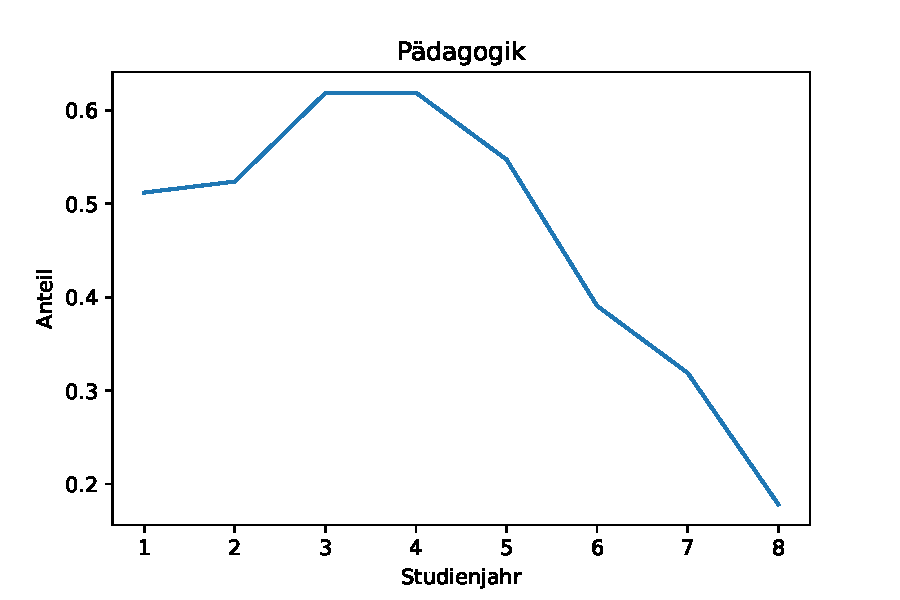
\includegraphics[width = 0.5\columnwidth]{pad1.pdf}
  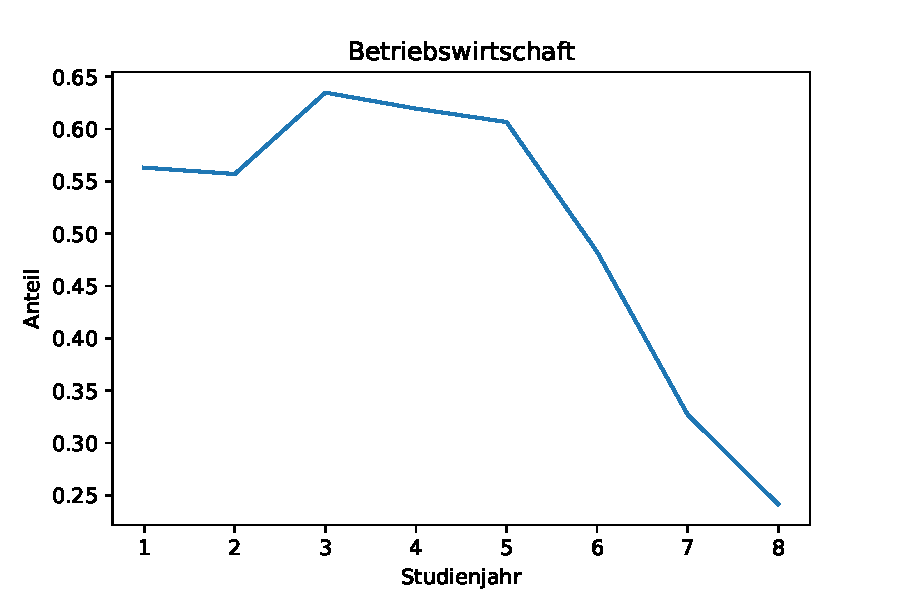
\includegraphics[width = 0.5\columnwidth]{bwl1.pdf}
  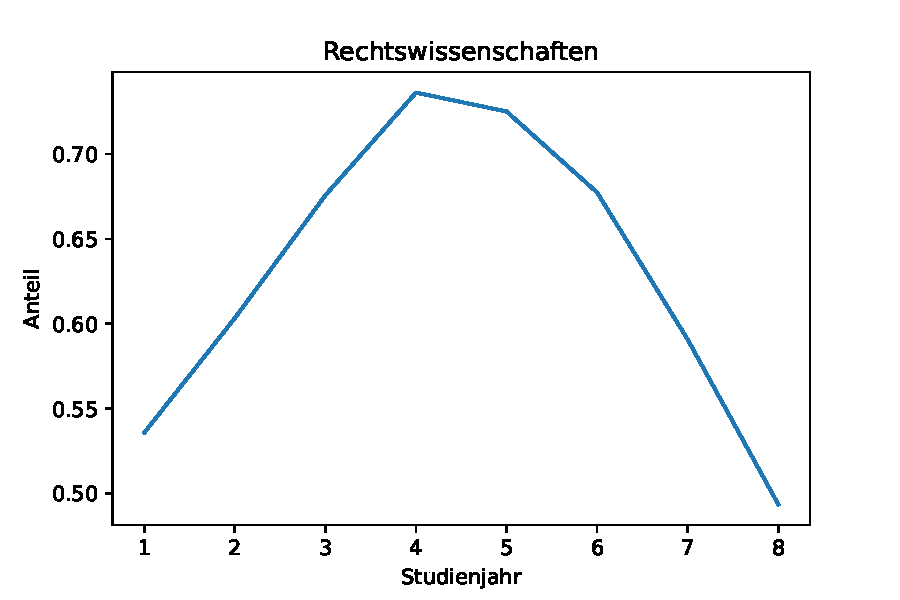
\includegraphics[width = 0.5\columnwidth]{jus1.pdf}
  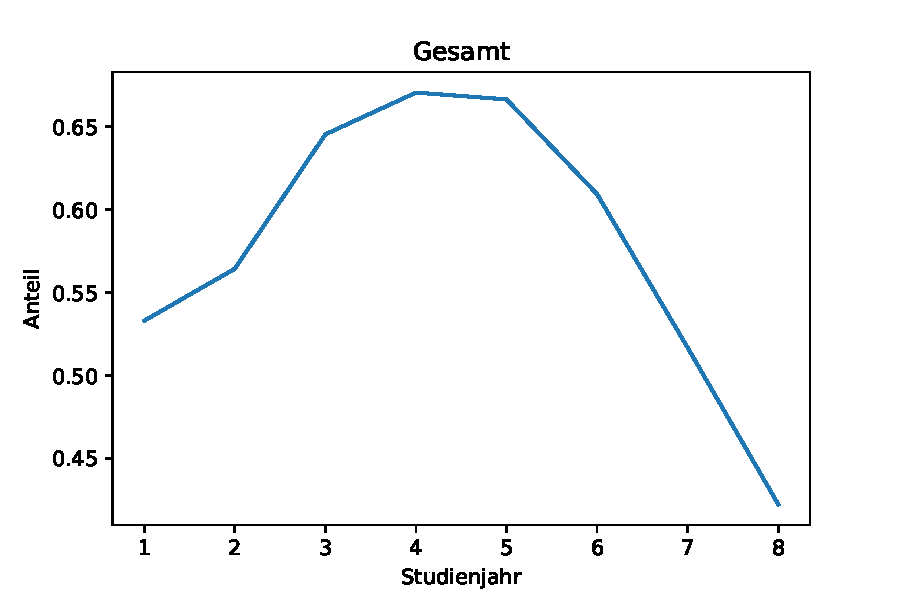
\includegraphics[width = 0.5\columnwidth]{ges1.pdf}
  \caption[Anteil an pr\"ufungsaktiven Studierenden nach Studienjahr und -richtung]{Der Anteil an pr\"ufungsaktiven Studierenden an insgesamt Studierenden, die noch bis ins jeweilige
    Studienjahr verblieben sind. In der Grafik \textit{Gesamt} wird ein gewichteter
    Anteil nach Studienrichtung gezeigt.}
\end{figure}

Eine Grundannahme in s\"amtlichen erprobten Ans\"atzen ist, dass Studierende, von denen man Anzahl und Merkmalskombinationen genau kennt, auch in einem Zeitrahmen von
drei Jahren in der Zukunft auch noch einen beachtlichen Anteil an den pr\"ufungsaktiven Studierenden bilden werden. Diese Annahme wird gest\"utzt, weil man, wie in \hyperref[fig:abb2]{Abbildung 1.2}
dargestellt, sieht, dass der Anteil an pr\"ufungsaktiven Studierenden aus h\"oheren Studienjahren tats\"achlich gro{\ss} ist. W\"are das nicht der Fall, m\"usste man sich nicht mit
P1 auseinandersetzen.

\begin{figure}[ht]
  \label{fig:abb2}
  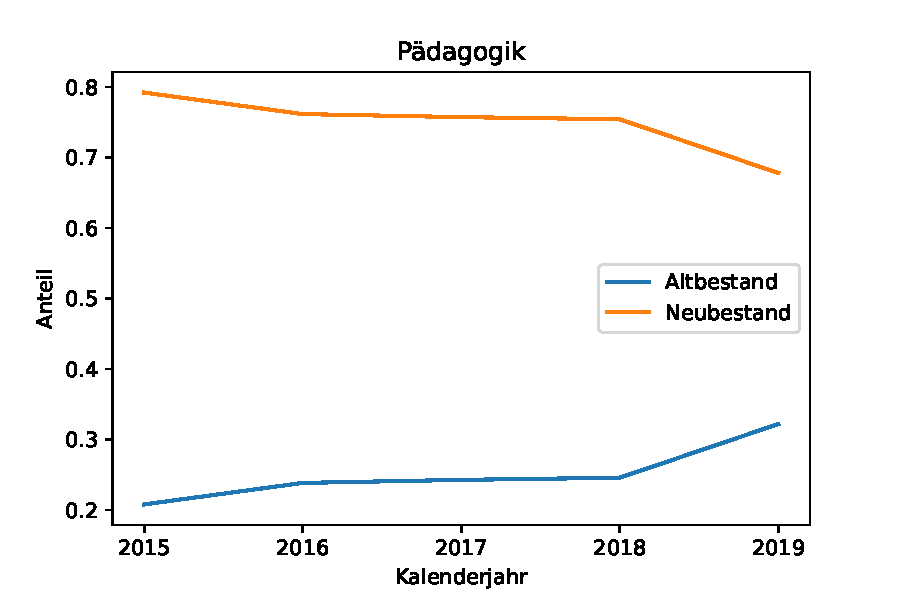
\includegraphics[width = 0.5\columnwidth]{pad2.pdf}
  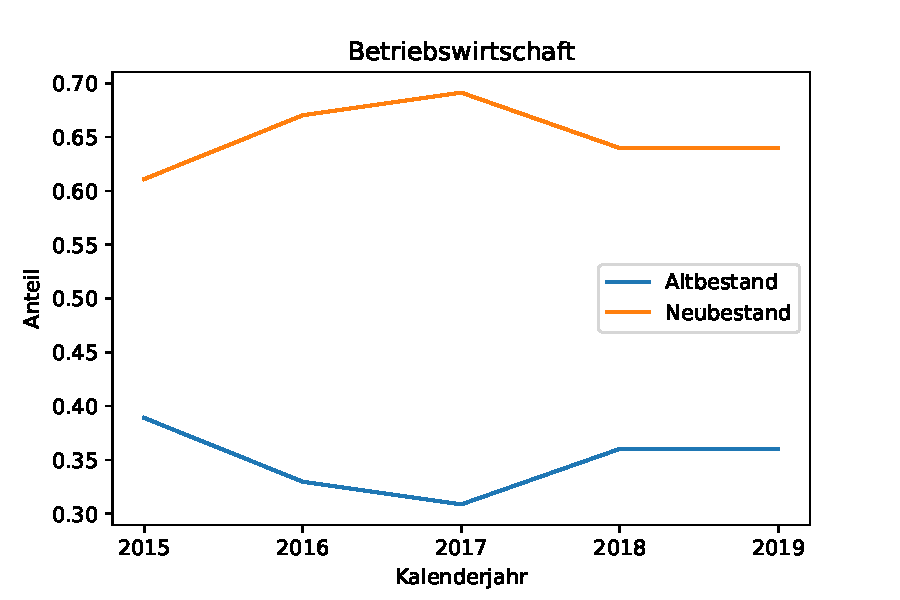
\includegraphics[width = 0.5\columnwidth]{bwl2.pdf}
  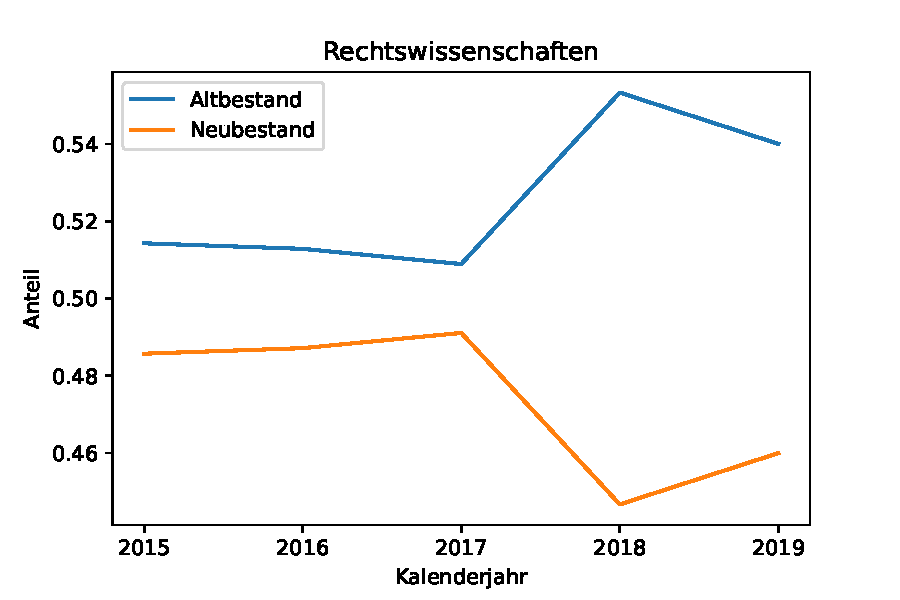
\includegraphics[width = 0.5\columnwidth]{jus2.pdf}
  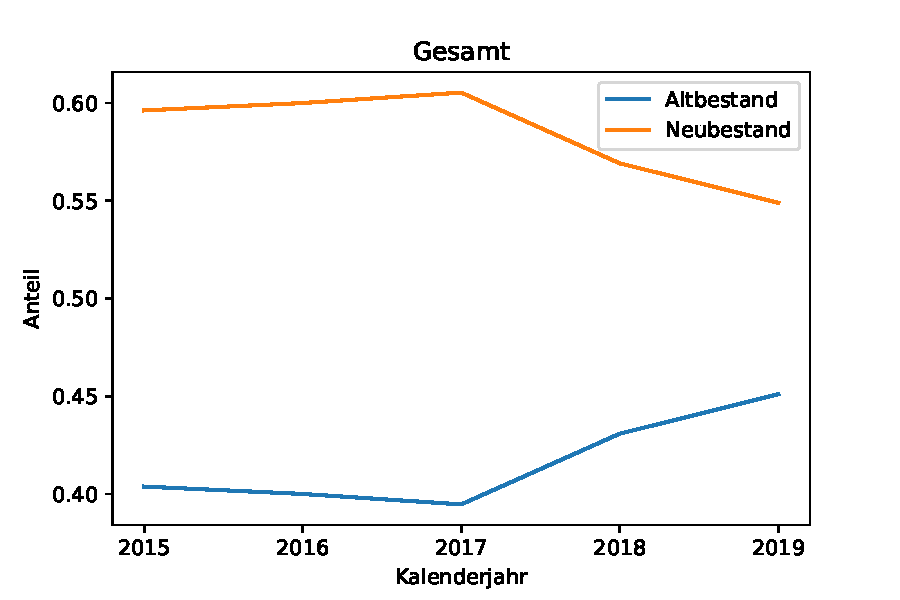
\includegraphics[width = 0.5\columnwidth]{ges2.pdf}
  \caption[Anteile des Neu- und Altbestandes an aktiven Studierenden]{Der Anteil an prüfungsaktiven Studierenden, welcher bereits im vierten oder einem höheren
    Studienjahr vorliegt (Altbestand) und der Anteil, welcher erst im dritten oder einem niedrigeren Studienjahr ist (Neubestand).Die Grafik \textit{Gesamt} stellt einen gewichteten
    Anteil nach Studienrichtung dar.}
\end{figure}

Weil man sich in P2 mit den zuk\"unftigen Studienbeginnern besch\"aftigt, ist es wichtig zu wissen, wie sich diese Zahl im Verlauf der Zeit ver\"andert. In
\hyperref[fig:abb3]{Abbildung 1.3} sieht man, wie sich diese Zahlen je nach Studienrichtung und als Zusammenfassung aller Studienrichtungen ver\"andern.

\begin{figure}[ht]
  \label{fig:abb3}
  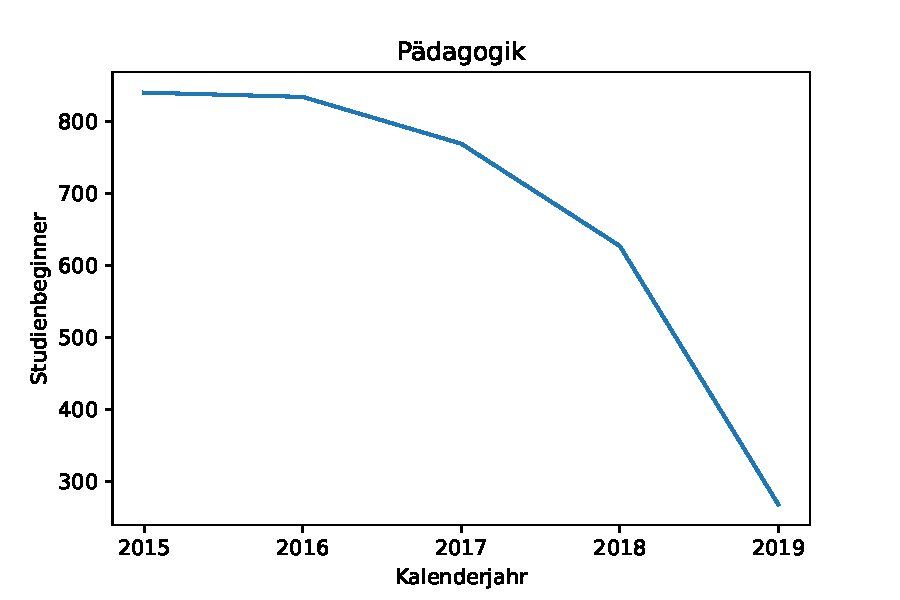
\includegraphics[width = 0.5\columnwidth]{pad3.pdf}
  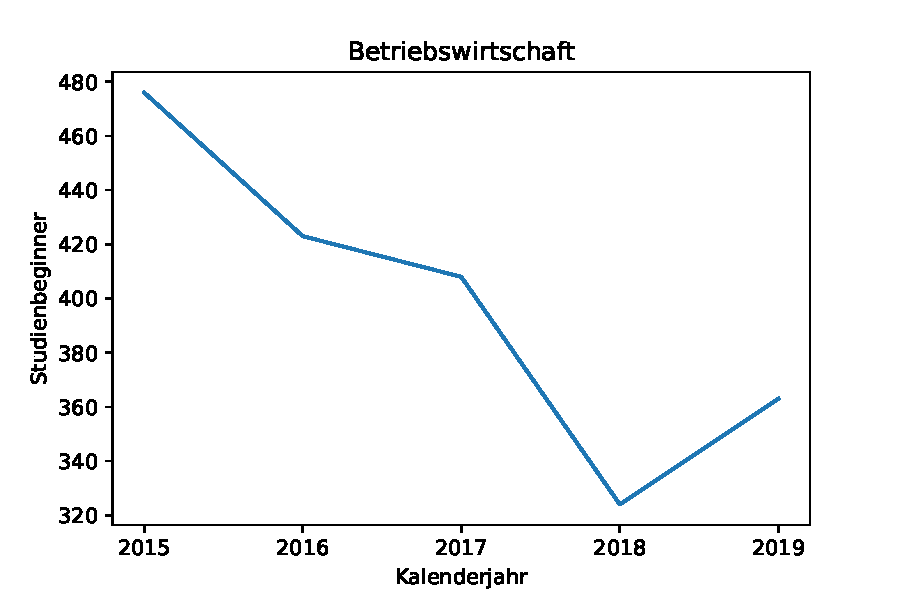
\includegraphics[width = 0.5\columnwidth]{bwl3.pdf}
  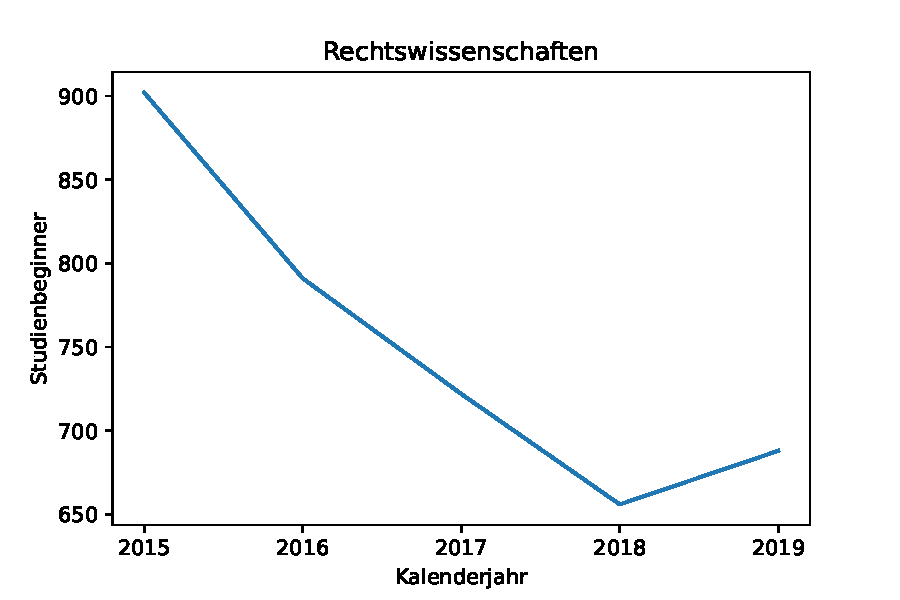
\includegraphics[width = 0.5\columnwidth]{jus3.pdf}
  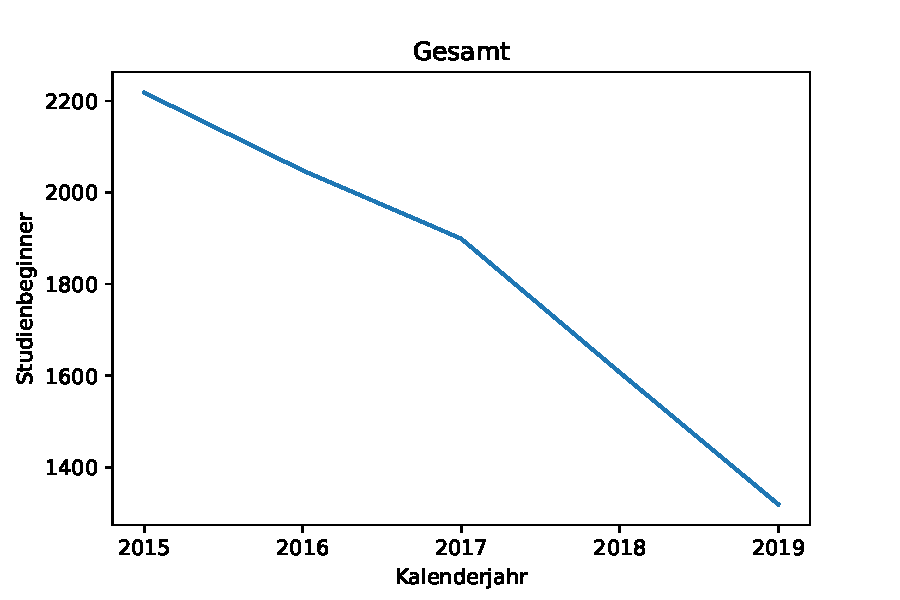
\includegraphics[width = 0.5\columnwidth]{ges3.pdf}
  \caption[Anzahl der Studienbeginner nach Fach und Kalenderjahr]{Hier werden die Anzahlen an Studienbeginnern je nach Fach und Kalenderjahr dargestellt.}
\end{figure}

Um einen besseren Einblick in die Zahlen der Studierenden nach Studienjahr und Kalenderjahr zu bekommen, sind in \hyperref[tab:numbers]{Tabelle 1.2} s\"amtliche
Zahlen nach Studienrichtung angef\"uhrt.

\begin{table}[ht]
  \caption{\label{tab:numbers} Anzahl der Studierenden nach Studienrichtung, Kalenderjahr und Studienjahr}
  \begin{tabular}{ p{1.5cm} p{1cm} p{1cm} p{1cm} p{1cm} p{1cm} p{1cm} p{1cm} p{1cm} p {1.5cm} }
    \toprule
                    &     & Jahr 1 & Jahr 2 & Jahr 3 & Jahr 4 & Jahr 5 & Jahr 6 & Jahr > 7 & \textbf{Gesamt} \\
    \midrule
    \multirow{3}{3em}{2015$/$16}
                    & JUS & 902    & 667    & 475    & 409    & 397    & 382    & 1253     & 4485            \\
                    & BWL & 476    & 353    & 231    & 355    & 153    & 104    & 399      & 2071            \\
                    & PAD & 804    & 567    & 415    & 270    & 115    & 48     & 115      & 2370            \\
    \midrule
    \multirow{3}{3em}{2016$/$17}
                    & JUS & 791    & 668    & 479    & 404    & 363    & 333    & 1285     & 4323            \\
                    & BWL & 423    & 357    & 308    & 177    & 181    & 73     & 374      & 1893            \\
                    & PAD & 834    & 538    & 419    & 282    & 122    & 57     & 126      & 2378            \\
    \midrule
    \multirow{3}{3em}{2017$/$18}
                    & JUS & 722    & 579    & 501    & 401    & 368    & 291    & 1257     & 4119            \\
                    & BWL & 408    & 314    & 286    & 228    & 75     & 83     & 324      & 1718            \\
                    & PAD & 769    & 578    & 419    & 279    & 124    & 68     & 139      & 2376            \\
    \midrule
    \multirow{3}{3em}{2018$/$19}
                    & JUS & 656    & 541    & 413    & 413    & 360    & 294    & 1153     & 3830            \\
                    & BWL & 324    & 292    & 254    & 202    & 113    & 49     & 270      & 1504            \\
                    & PAD & 627    & 453    & 444    & 268    & 120    & 56     & 128      & 2106            \\
    \midrule
    \multirow{3}{3em}{2019$/$20}
                    & JUS & 688    & 502    & 386    & 363    & 367    & 296    & 1113     & 3715            \\
                    & BWL & 363    & 242    & 244    & 192    & 96     & 66     & 231      & 1434            \\
                    & PAD & 268    & 415    & 335    & 292    & 122    & 50     & 138      & 1620            \\
    \midrule
    \multirow{3}{3em}{Gesamt Jahre}
                    & JUS & 3759   & 2957   & 2254   & 1990   & 1855   & 1596   & 6061     & 20472           \\
                    & BWL & 1994   & 1558   & 1323   & 1154   & 618    & 375    & 1598     & 8620            \\
                    & PAD & 3302   & 2551   & 2032   & 1391   & 603    & 279    & 656      & 10850           \\
    \midrule
    \textbf{Gesamt} &     & 9091   & 7066   & 5609   & 4535   & 3076   & 2250   & 8315     & 39942           \\

    \bottomrule
  \end{tabular}

\end{table}




\begin{figure}[ht]
  \label{fig:abb4}
  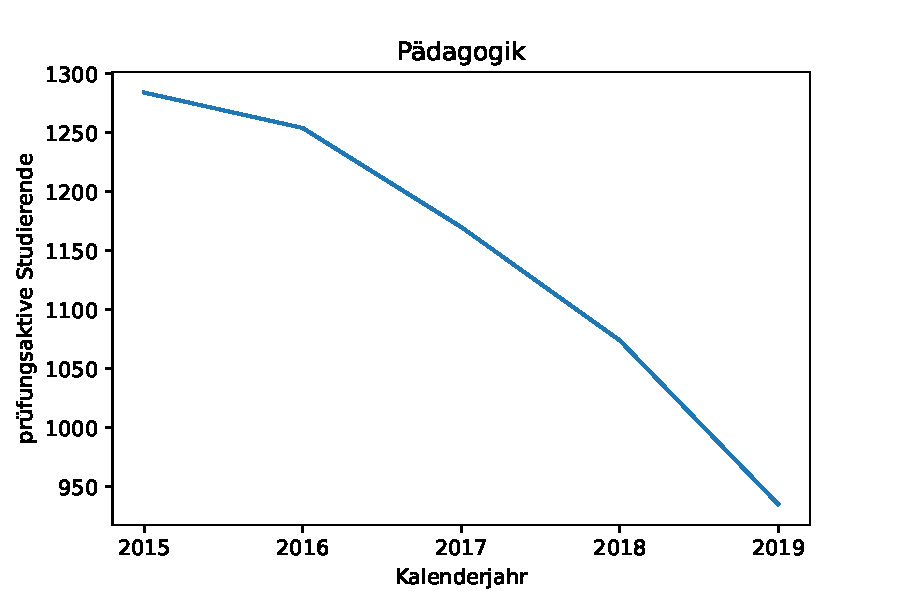
\includegraphics[width = 0.5\columnwidth]{pad4.pdf}
  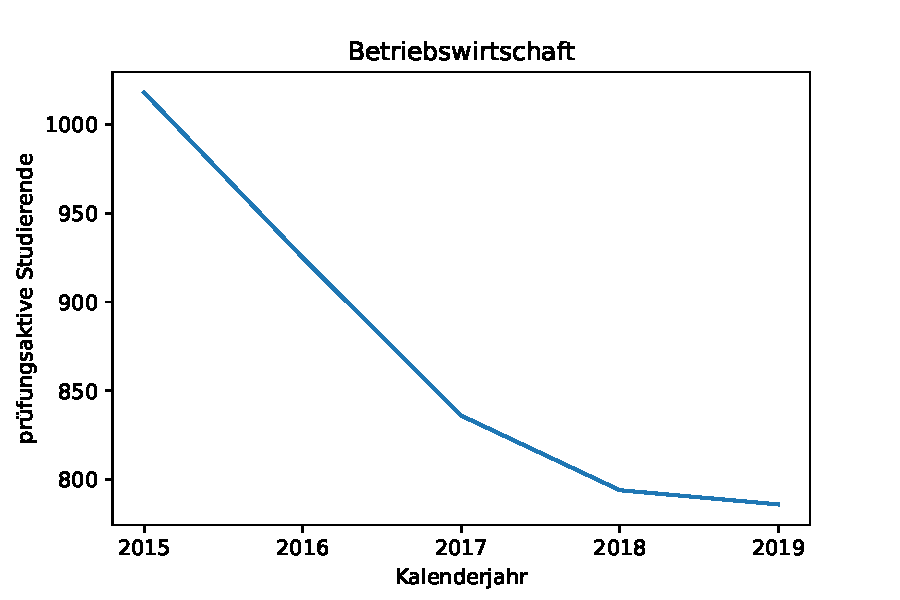
\includegraphics[width = 0.5\columnwidth]{bwl4.pdf}
  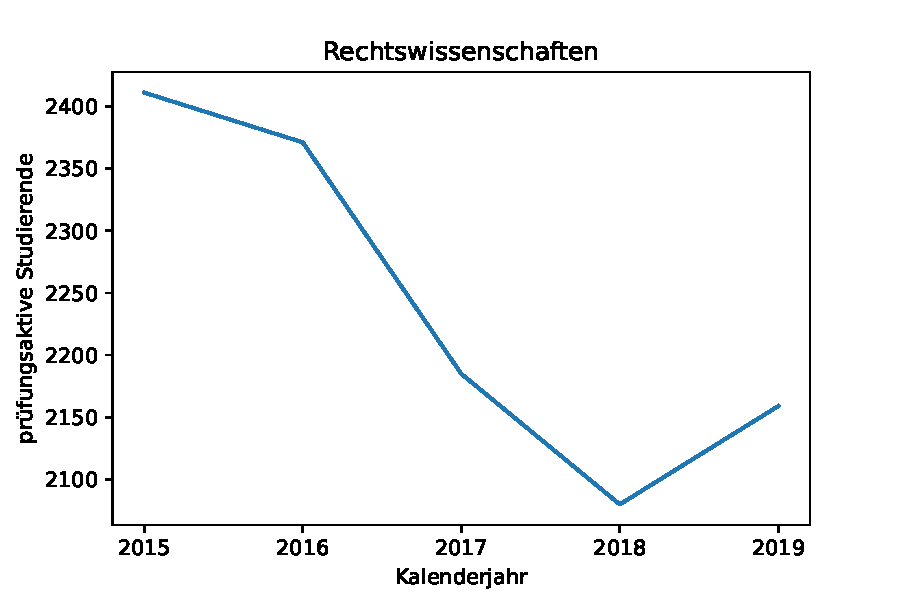
\includegraphics[width = 0.5\columnwidth]{jus4.pdf}
  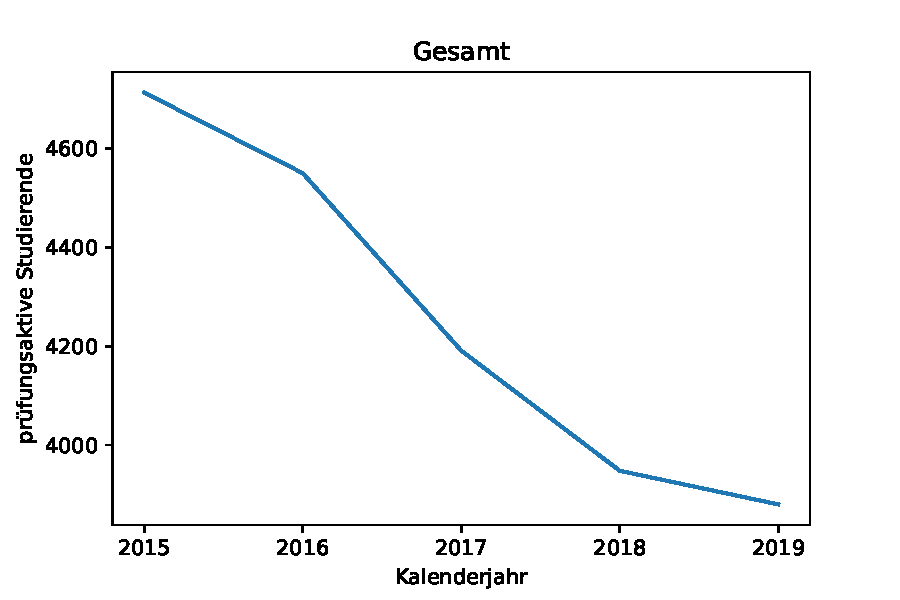
\includegraphics[width = 0.5\columnwidth]{ges4.pdf}
  \caption[prüfungsaktive Studierende nach Kalenderjahr]{Hier wird die Anzahl aller prüfungsaktiven Studierenden nach Kalenderjahr dargestellt. Das
    ist jene Zahl, die anschließend in der Zukunft geschätzt werden soll.}
\end{figure}


% \begin{figure}[ht]
%   \label{fig:abb5}
%   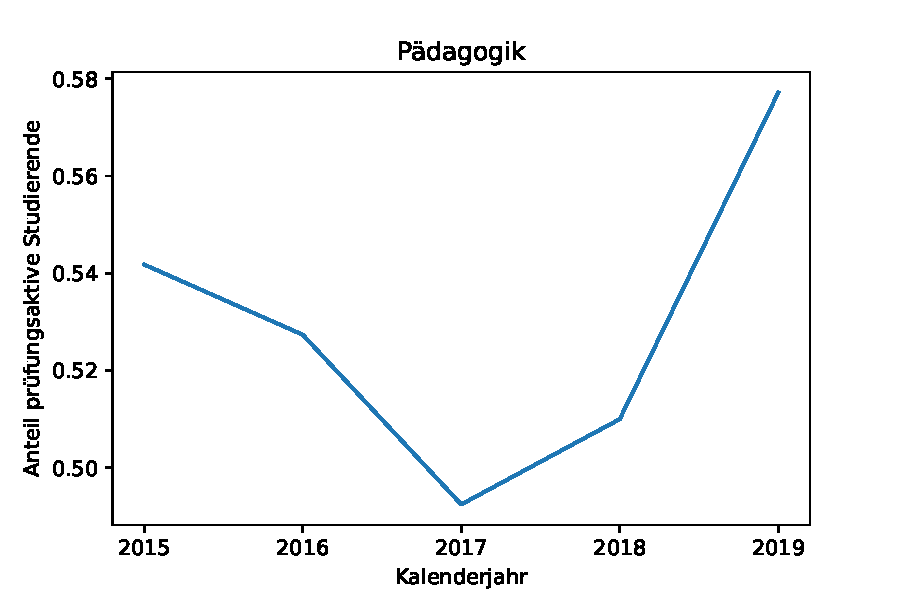
\includegraphics[width = 0.5\columnwidth]{pad5.pdf}
%   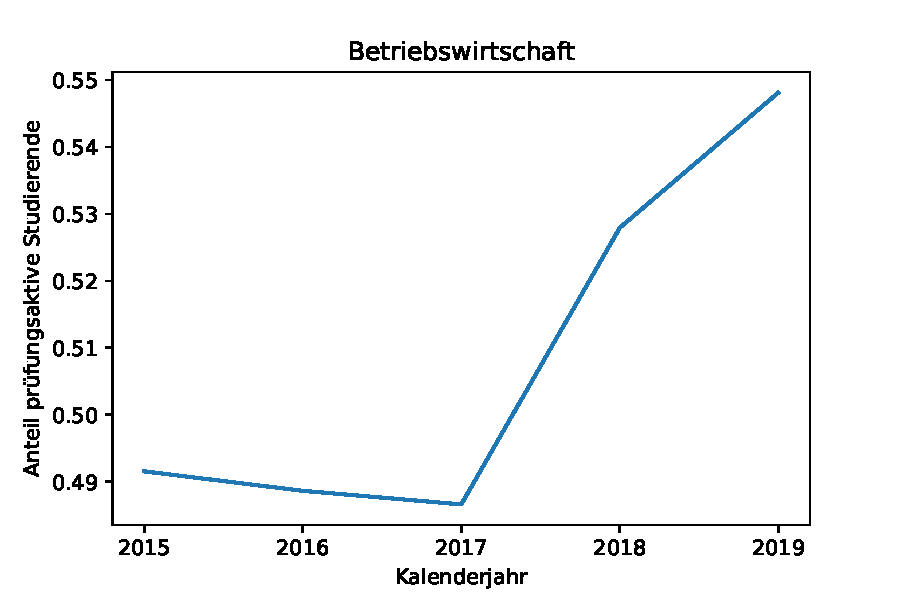
\includegraphics[width = 0.5\columnwidth]{bwl5.pdf}
%   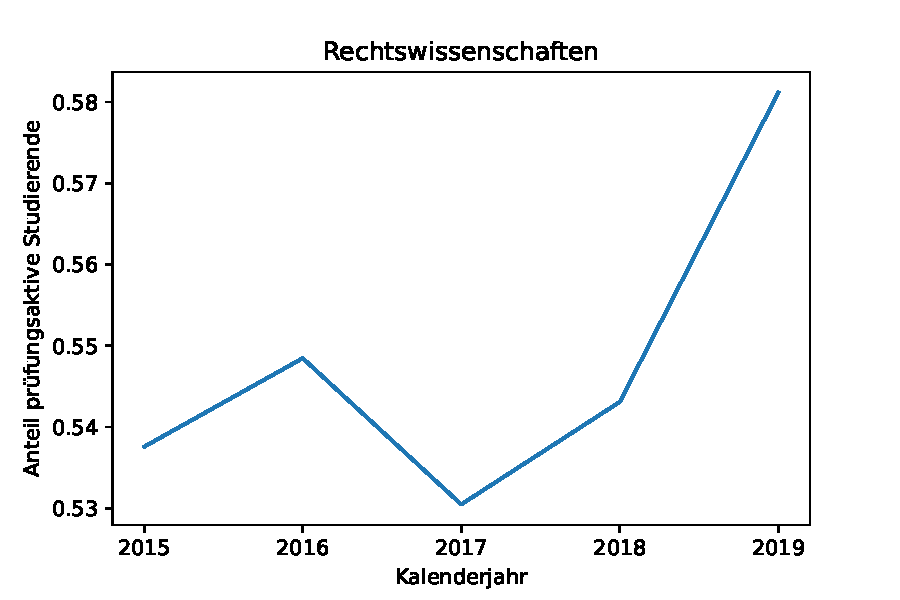
\includegraphics[width = 0.5\columnwidth]{jus5.pdf}
%   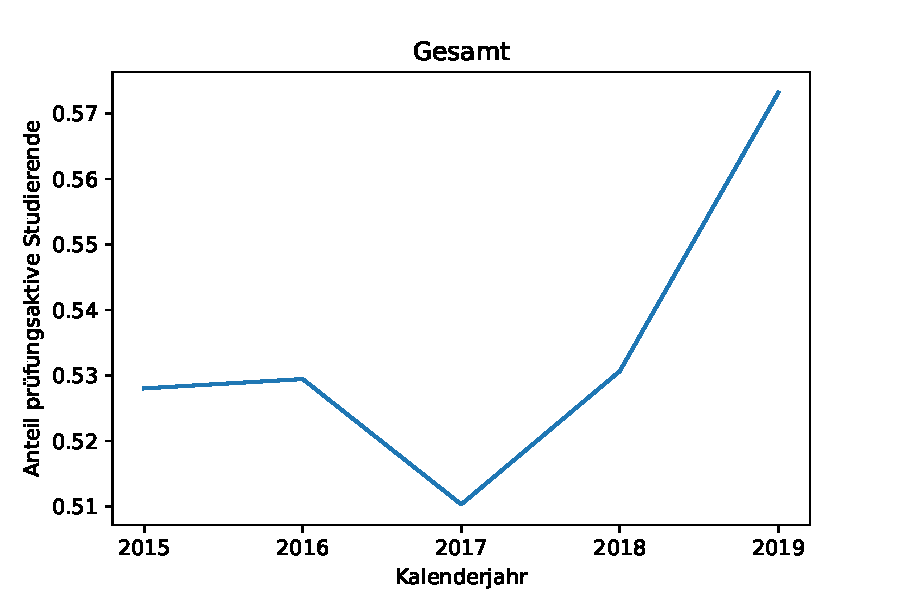
\includegraphics[width = 0.5\columnwidth]{ges5.pdf}
%   \caption[Anteil der prüfungsaktiven Studierenden nach Kalenderjahr]{Hier wird der Anteil an prüfungsaktiven Studierenden nach Kalenderjahr dargestellt.}
% \end{figure}












\chapter{Methoden und Modelle}

% Methoden und Modelle

In diesem Abschnitt werden L\"osungsans\"atze f\"ur P1 und P2 und deren Implementierung vorgestellt.
Weiters werden die unterschiedlichen Machine Learning Modelle erkl\"art, die in den L\"osungsans\"atzen verwendet werden.
Abschlie{\ss}end wird dargelegt, wie die unterschiedlichen Ans\"atze und auch die einzelnen Machine Learning Modelle
verglichen und ausgewertet werden.

% Problem 1

\section{Ans\"atze f\"ur Problem 1}
P1 stellt die Sch\"atzung der Anzahl der pr\"ufungsaktiven Studierenden im Jahr $t = 3$ aus den bestehenden Studierenden im Jahr $t = 0$ dar.
Von diesen Studierenden kennt man die Anzahl und die Merkmalskombination jeder einzelnen Person.

\subsection{Ansatz 1}
\label{sec:appr1}
In Ansatz 1 versucht man die Pr\"ufungsaktivit\"at der Studierenden Jahr f\"ur Jahr zu modellieren und so viel Information wie m\"oglich weiterzuverwenden.
Insbesondere soll f\"ur das jeweilige darauffolgende Studienjahr der ECTS-Wert vorhergesagt werden. Viele weitere Eigenschaften der studierenden Person
k\"onnen dann aus diesem ECTS-Wert abgeleitet werden.

Der Ausgangspunkt ist, dass sich für alle $S_i \in Z^{(t)}$ der erste Eintrag $E_i^{(1)}$ (aktuelles Studienjahr) um eins erhöht.
Nun wird versucht eine Funktion zu finden, welche jeder studierenden Person $S_i \in Z^{(t)}$ einen passenden ECTS-Wert vorhersagt.
Somit kann f\"ur diese Person der \"Ubergang nach $Z_{alt}^{(t+1)}$ beschrieben werden und man hat alle Eintr\"age zur Verf\"ugung, die
man auch von den zuvor gegebenen Daten hatte. Der Ansatz besteht darin, die Funktion wie folgt zu bilden.

$$
  F(S_i)=
  \left\{
  \begin{array}{lr}
    h_1(S_i), & \text{für }E_i^{(1)} = 1    \\
    h_2(S_i), & \text{für }E_i^{(1)} \geq 2 \\
  \end{array}
  \right.
$$

Die Funktionen $h_1$ und $h_2$ sind Sch\"atzfunktionen, die einer gewissen Merkmalskombination einer studierenden Person in einem Studienjahr einen
ECTS-Wert zuordnen.

Studierende im ersten Studienjahr werden gesondert betrachtet, weil f\"ur sie keine Eintr\"age mit ECTS-Werten vorhanden sind.
Aufgrund dessen gibt es f\"ur sie weniger Inputwerte.
Nun gibt es verschiedene M\"oglichkeiten $h_1$ und $h_2$ auszuwählen. In dieser Arbeit
werden folgende Machine Learning Modelle ausprobiert:

\begin{itemize}
  \item Multiple Lineare Regression
  \item Random Forest Modelle
  \item Support Vector Machines
  \item K\"unstliche neuronale Netzwerke
\end{itemize}

Jedes Modell bekommt als Input die Eigenschaften einer studierenden Person. Anhand dieser Eigenschaften ist es das Ziel, m\"oglichst genau
vorherzusagen, wie viele ECTS diese Person im kommenden Studienjahr erreichen wird.

Je nachdem wie gut die einzelnen Vorhersagefunktionen für die vorliegende Problemstellung funktioneren
und angepasst werden können, w\"ahlt man anhand einer Metrik, die sp\"ater beschrieben wird, jenes Modell aus, welches
am besten die jeweiligen ECTS-Werte vorhersagen kann.
Wichtig ist, dass jedes dieser Modelle eine Regression der ECTS f\"ur das aktuelle Studienjahr
durchf\"uhrt. Aufgrund der gesch\"atzten ECTS kann dann entschieden werden, ob die Person
pr\"ufungsaktiv ist oder nicht. Die Regression der ECTS, anstelle einer Klassifikation nach
\textit{pr\"ufungsaktiv} oder \textit{pr\"ufungsinaktiv} wird deshalb gew\"ahlt, weil man im darauffolgenden Studienjahr diese
gesch\"atzten ECTS als Input f\"ur die Sch\"atzung verwenden will.


Um die tats\"achliche Sch\"atzung der pr\"ufungsaktiven Studierenden in drei Jahren durchzuf\"uhren, werden f\"ur die
aktuellsten Daten die ECTS jeweils im darauffolgenden Jahr vorhergesagt. Das wird f\"ur drei Jahre in der Zukunft durchgef\"uhrt.
Dabei baut man ab dem zweiten vorhergesagten Jahr
bereits auf einer Sch\"atzung auf. Danach kann man f\"ur jeden Eintrag anhand der gesch\"atzten ECTS entscheiden, ob er im Jahr $t = 3$ pr\"ufungsaktiv sein wird oder nicht.

Weil man Vorhersagen aufgrund von bereits gesch\"atzten Daten durchf\"uhrt, kann es zu einer Fehlerfortpflanzung kommen.
Es gilt nun herauszufinden, ob sich diese in Grenzen h\"alt oder ob sich dieser Ansatz als unbrauchbar erweist.





\subsection{Ansatz 2}
\label{sec:appr2}

Im zweiten Ansatz beachtet man, dass es Eigenschaften gibt, die sich w\"ahrend der gesamten Studienzeit nicht verändern. Alle ver\"anderlichen Merkmale,
wie beispielsweise \textit{ECTS im Jahr zuvor}, werden nicht betrachtet.
Diese Eigenschaften und deren Ausprägungen sind:

\begin{itemize}
  \item Geschlecht (männlich, weiblich)
  \item Schulbesuch (AHS, BHS, andere)
  \item Herkunft (Steiermark, Österreich ohne Steiermark, \\
        Deutschland, Ausland ohne Deutschland)
  \item Studienrichtung (Rechtswissenschaften, Betriebswirtschaft, P\"adagogik)
\end{itemize}

Somit ergeben sich 72 verschiedene Kombinationen. Man kann nun alle 72 verschiedenen
Kombinationen betrachten. Da alle anderen Eigenschaften nicht betrachtet werden, unterscheiden sich die Kombinationen in den
ausstehenden Eigenschaften nicht und man kann für jede Kombination gleich vorgehen.

Es wird von zeitlich ver\"anderbaren Zuständen $Z^{(t)}$ ausgegangen, wobei jeder dieser
Zustände einer Menge von Studierenden entspricht. Anstatt eine Funktion von $Z^{(t)}$ nach $Z_{alt}^{(t+1)}$
zu verwenden, ist hier der Ansatz, einen stochastischen Prozess $X = (X_r)_{r \in \{ 0,1, \dots, k \} }$ zu definieren, welcher einzelne Studierende \"uber
die Zeit ihres Studiums $r \in \{0,1, \dots , k\}$ beschreibt.

Wichtig ist hier die Unterscheidung zwischen den Zuständen $Z^{(t)}$ und dem Prozess $X = (X_r)_{r \in \{ 0,1, \dots, k \} }$.
$Z^{(t)}$ gibt die Menge der Studierenden zur gewünschten Zeit $t$ ab einem festgelegten Zeitpunkt an.
$X_r$ gibt die Zustände der einzelnen Studierenden im jeweiligen Studienjahr $r$ an, indem sich die studierende Person gerade befindet.
Das bedeutet, dass der Prozess $X$ auf der Ebene eines jeden Studierenden abläuft, wohingegen
die Zust\"ande $Z^{(t)}$ die aggregierte Menge der gesamten Studierenden im Jahr $t$ beschreibt.

Eine weitere Annahme in diesem Ansatz ist die \textit{Markov Eigenschaft} des Prozesses $X_r$. Sie besagt, dass der Zustand, in dem sich die studierende Person
befindet, die gesamte Information f\"ur den weiteren Verlauf der studierenden Person im Prozess $X$ beinhaltet \cite[Seite 340]{tsitsiklis}.

Der Prozess $X = (X_r)_{r \in \{ 0,1, \dots, k \} }$ hat ab den Jahren $r \geq 1$ folgende m\"ogliche Zust\"ande:
\begin{itemize}
  \item \textbf{a}: steht f\"ur Studierende die zwar pr\"ugungsaktiv waren, aber nicht f\"ur das kommende Jahr inskribiert sind. Das hei{\ss}t aufgrund eines Abschlusses, eines Abbruchs oder aufgrund einer Pausierung des Studiums.
  \item \textbf{b}: steht f\"ur Studierende die pr\"ufungsinaktiv waren, aber nicht f\"ur das kommende Jahr inskribiert sind. Das hei{\ss}t aufgrund eines Abbruches oder aufgrund einer Pausierung des Studiums.
  \item \textbf{c}: steht f\"ur Studierende die pr\"ufungsaktiv waren, und auch f\"ur das n\"achste Jahr inskribiert sind.
  \item \textbf{d}: steht f\"ur Studierende die pr\"ufungsinaktiv waren, aber dennoch weiterhin f\"ur das n\"achste Jahr inskribiert sind.
\end{itemize}

Jede studierende Person muss sich in einem dieser Zust\"ande befinden. Von dort ausgehend gibt es f\"ur diese Person gewisse Wahrscheinlichkeiten,
in welchem Zustand sie im kommenden Jahr sein wird.
Aus diesem Grund müssen alle Übergangswahrscheinlichkeiten $p_r^{(xy)}$ f\"ur eine bestimmte Kategorie
abgeschätzt werden, wobei $x \in \{c, d \}$ und $y \in \{a, b, c, d\}$ ist.
Jeder Studierende dieser Kombination muss sich in einem dieser Zustände befinden und hat dann die
angegebenen Übergangswahrscheinlichkeiten für den neuen Zustand im kommenden Studienjahr. \hyperref[fig:prozess]{ Abbildung 2.1} beschreibt den Prozess $X$ grafisch.

\begin{figure}[ht]
  \label{fig:prozess}
  \begin{center}
    \tikzfig{fig1}
  \end{center}
  \caption[Grafische Darstellung des zweiten Modells]
  {Der Prozess $X = (X_r)_{r \in \{ 0,1, \dots, k \} }$ ist hier für den Studienbeginn und die ersten vier Studienjahre $X_0, X_1, X_2, X_3, X_4$ dargestellt.
    $X_r$ eines jeweiligen Studierenden im Jahr $r$ kann folgende Werte annehmen: $X_r \in \{a, b, c, d\}$.
    Die Übergangswahrscheinlichkeiten sind entlang der blauen und schwarzen Linien zu erkennen.}
\end{figure}

Dieser Ansatz profitiert von der Eigenschaft der Problemstellung, dass nur die absolute H\"aufigkeit an pr\"ufungsaktiven Studierenden auf aggregierter Ebene
gefragt ist. Es ist nicht wichtig zu wissen, ob eine Studentin oder ein Student in einem bestimmten Studienjahr pr\"ufungsaktiv war oder nicht.
Somit konvergiert die Sch\"atzung der pr\"ufungsaktiven Studierenden
fast sicher gegen die tats\"achliche Anzahl der pr\"ufungsaktiven Studierenden, wenn die Anzahl der gesch\"atzen Personen gro{\ss} wird. Diese Bedingung ist in dieser Problemstellung
erf\"ullt.

\subsection{Ansatz 3}
\label{sec:appr3}
Im dritten Ansatz wird versucht, passende \"Ubergangswahrscheinlichkeiten zu finden. Man versucht die Wahrscheinlichkeit zu finden, mit der eine studierende Person zu einem
gewissen Zeitpunkt $t$ in der Zukunft pr\"ufungsaktiv sein wird.
Zum Beispiel wird die Wahrscheinlichkeit gesucht, mit der eine studierende Person \textit{in drei Jahren in der Zukunft} pr\"ufungsaktiv sein wird oder nicht.


In Ansatz 2 wurde jede studierende Person auf vier Eigenschaften beschr\"ankt.
In diesem Ansatz sollen mehr Eigenschaften genutzt werden. Das bedeutet, es werden auch die Informationen
\"uber absolvierte ECTS aus der Vergangenheit verwendet.


Um dieses Ziel zu erreichen, werden Machine Learning Modelle verwendet, welche grunds\"atzlich zur Klassifizierung dienen.
Diese Klassifizierung wird mithilfe einer berechneten Wahrscheinlichkeit und eines manuell bestimmten Schwellwertes durchgef\"uhrt.
Da man bei der vorliegenden Problemstellung jedoch keine exakte Klassifizierung ben\"otigt, sondern ausschlie{\ss}lich die Anzahl an
pr\"ufungsaktiven Studierenden wissen will, wird nur die berechnete Wahrscheinlichkeit verwendet, ohne zu klassifizieren. Man summiert f\"ur alle 
Studierenden deren gesch\"atzte Wahrscheinlichkeiten pr\"ufungsaktiv zu sein auf und erh\"alt somit die erwartete Anzahl an pr\"ufungsaktiven Studierenden.

Es ist ein Vorteil neben vielen unterschiedlichen Klassen, welche durch diskrete Eigenschaften entstehen (analog zu Ansatz 2), auch kontinuierliche Datenpunkte von
Studierenden verwenden zu k\"onnen. Somit werden beispielsweise auch Eigenschaften wie \textit{\glqq kumulierte ECTS\grqq{}} und \textit{\glqq ECTS im Jahr zuvor\grqq{}} verwendet. Damit wird erreicht, dass
m\"oglichst viel Information verwendet wird, was bei einer reinen Wahrscheinlichkeitsberechnung wie in Ansatz 2 nicht m\"oglich ist.

Es wird eine Funktion $F_t(\cdot)$ gesucht, welche f\"ur alle Studierenden eine Wahrscheinlichkeit $p_t$ ausgibt, mit der
sie im Jahr $t$ pr\"ufungsaktiv sein werden oder nicht. Es braucht f\"ur unterschiedliche Zeitspannen mehrere Funktionen, die in ihrem Aufbau gleich sind.
Das bedeutet, man muss f\"ur jede Zeitspanne von $t$ Jahren, die unterschiedlich lang sein kann, eine neue Funktion trainieren.
Die Vorhersagefunktionen sind wie folgt aufgebaut:

$$
  F_t(S_i)=
  \left\{
  \begin{array}{lr}
    h_1^{(t)}(S_i), & \text{für }E_i^{(1)} = 1    \\
    h_2^{(t)}(S_i), & \text{für }E_i^{(1)} \geq 2 \\
  \end{array}
  \right.
  \in (0,1)
$$

Die Unterscheidung in $h_1$ und $h_2$ ist wieder notwendig, da man im ersten Studienjahr noch keine Informationen \"uber ECTS in den vorangegangen Jahren hat.
Weiters ist der Output der Funktion eine Wahrscheinlichkeit $p_t \in (0,1)$.

Es werden folgende Machine Learning Modelle in diesem Ansatz verwendet:
\begin{itemize}
  \item Logistische Regression
  \item Support Vector Machine Modelle
  \item Random Forest Modelle
  \item K\"unstliche Neuronale Netzwerke
\end{itemize}

Es wird anschlie{\ss}end das Modell ausgew\"ahlt, welches nach einer unten beschriebenen Metrik, die Anzahl der pr\"ufungsaktiven Studierenden
im Jahr $t = 3$, am besten vorhersagen kann.

Um eine Vorhersage in der Praxis durchzuf\"uhren, werden die aktuellsten Daten verwendet und f\"ur jede studierende Person wird die
Wahrscheinlichkeit gesch\"atzt, mit der sie im Jahr $t=3$ pr\"ufungsaktiv sein wird. Danach werden alle gesch\"atzten Wahrscheinlichkeiten summiert und
man erh\"alt den Erwartungswert an pr\"ufungsaktiven Studierenden in drei Jahren.






% Problem 2

\section{Ans\"atze f\"ur Problem 2}
P2 stellt die Sch\"atzung der pr\"ufungsaktiven Studierenden von zuk\"unftigen Studienbeginnern in drei Jahren in der Zukunft dar. Von diesen Studierenden
kennt man weder Anzahl noch Merkmalskombinationen. Es handelt sich jedoch immer um Neuinskripenten, die hinzukommen.

\subsection{Ansatz 1}
Im ersten Ansatz wird versucht die Zahl aller neu inskribierenden Personen in den folgenden zwei Kalenderjahren zu sch\"atzen. Hierzu wird probiert, mittels einer Regression aus
Daten von vergangen Jahren, den Trend der Anzahl von neu inskribierenden Personen fortzusetzen. Diese Sch\"atzung der Anzahl an neu hinzukommenden Studierenden beinhaltet
eine gewisse Unsicherheit, da die Anzahl an neu inskribierenden Personen von vielen unterschiedlichen Faktoren abh\"angig sein kann, von denen man 
aber keine Informationen zur Verf\"ugung hat.

Wenn man einen Wert f\"ur die Anzahl der kommenden Studienbeginnerinnen und Studienbeginner gesch\"atzt hat, wird f\"ur ihre Merkmalskombination angenommen,
dass diese \textbf{gleich} mit jenen Merkmalskombinationen der neu inskribierenden Personen aus dem letzten gegebenen Jahr ist. Das bedeutet, man w\"ahlt eine Stichprobe mit Zur\"ucklegen 
der Gr\"o{\ss}e der gesch\"atzten Anzahl aus, welche aus den Merkmalen von Studienbeginner:innen aus dem letzten Jahr besteht, von denen man die Daten 
noch zur Verf\"ugung hat.

Nachdem man mit der gesch\"atzten Anzahl und den angenommen Merkmalskombinationen neue fiktive Studienbeginner:innen f\"ur die kommenden beiden Jahre erstellt hat, kann man
sch\"atzen, ob sie in einer gewissen Zeitspanne in der Zukunft pr\"ufungsaktiv sein werden oder nicht. Diese Sch\"atzung wird mit jener Methode durchgef\"uhrt, die
sich f\"ur P1 als erfolgreich erwiesen hat.


\subsection{Ansatz 2}
Im zweiten Ansatz werden die Studierenden nach folgenden unver\"anderbaren Merkmalen eingeteilt:

\begin{itemize}
  \item Geschlecht
  \item Herkunft
  \item besuchter Schultyp
  \item Studienrichtung
\end{itemize}

Dadurch ergeben sich 72 Kombinationen. Nun wird f\"ur jede dieser Kombinationen die Anzahl an zuk\"unftigen neu inskribierenden Personen mittels einer Regression aus Daten von
vergangenen Jahren versucht vorherzusagen. Das bedeutet, dass man in diesem Ansatz den Verlauf der Anzahl an neu inskribierenden Personen in jeder dieser Klassen versucht zu
ber\"ucksichtigen. Somit k\"onnen m\"ogliche Informationen von Klassen, die sich anders entwickeln als alle Klassen gemeinsam, beachtet werden. Jedoch ist die Sch\"atzung der
Anzahl an neu inskribierenden Personen aller Klassen mit Unsicherheit behaftet, da diese Zahl von vielen unterschiedlichen Faktoren abh\"angig sein kann, 
von denen man keine Informationen besitzt.

Nachdem man die Anzahl f\"ur alle Klassen gesch\"atzt hat, kann man eine Menge von fiktiven neu inskribierenden Personen bilden. Diese haben eine Merkmalskombination,
welche aus vier Merkmalen besteht. Nun kann man f\"ur jede fiktive Person sch\"atzen, ob sie in einer Zeitspanne in der Zukunft pr\"ufungsaktiv sein wird oder nicht.
Diese Vorhersage wird mit der Methode durchgef\"uhrt, welche sich f\"ur P1 als erfolgreich erwiesen hat.

% Machine Learning Modelle

\section{Machine Learning Modelle}
\label{sec:ml}

In P1 und P2 ist das Ziel, von Daten aus der Vergangenheit Informationen zu gewinnen, und diese f\"ur Vorhersagen in die Zunkunft zu verwenden.
Man versucht gewisse Muster in den Daten der Studierenden zu erkennen und anhand dieser eine Aussage \"uber deren Pr\"ufungsaktivit\"at in den kommenden Jahren zu treffen.
Diese Aufgabe ist f\"ur Menschen aufgrund der gro{\ss}en Anzahl an Daten schwer bew\"altigbar. Aus diesem Grund werden Machine Learning Modelle verwendet,
um dieses Ziel zu erreichen.

In dieser Arbeit werden ausschlie{\ss}lich Machine Learning Modelle verwendet, die man als \textit{supervised learning} bezeichnet.
Das bedeuted, man verf\"ugt \"uber Daten der Form $(\mathbf{x}_i, y_i)$ mit $i = 1,\dots,n$. Dabei stellt $\mathbf{x}_i \in \mathbb{R}^d$ den Eigenschaftsvektor
der Inputdaten und $y_i \in \mathbb{R}$ den bereits vorhandenen, tats\"achlichen Zielwert (oder Output) dar. Die Anzahl der Daten wird mit $n$ beschrieben. Alle Daten mit denen die
Sch\"atzfunktion optimal gebildet werden soll, werden als \textit{Trainingsdaten} bezeichnet.
Anhand der bekannten Outputs zu den jeweiligen Inputs kann das Modell durch einen Trainingsalgorithmus mit jedem Beispiel verbessert werden.
Man spricht dabei vom \textit{Training} des Modells \cite[Seiten 19 bis 25]{shalev}.

Das Ziel eines jeden Machine Learning Modells ist es, eine passende Regel zu erkennen, die nicht nur m\"oglichst viele Trainigsdaten richtig abbilden kann, sondern vor allem
gut auf neue, unbekannte Daten generalisiert \cite[Seite 371]{strang}. 

Die Inputdaten in der vorliegenden Problemstellung sind die Eigenschaftsvektoren der individuellen Studierenden in dem jeweiligen Studienjahr. Die Outputklassen oder
Outputwerte sind entweder die Klassifizierung \textit{pr\"ufungsaktiv}, \textit{nicht pr\"ufungsaktiv} oder die erreichten \textit{ECTS pro Jahr}.
In den folgenden Abs\"atzen wird Machine Learning genauer erkl\"art und formal beschrieben.



Wir bezeichnen $\mathcal{X}$ als Menge der Inputdaten und $\mathcal{Y}$ als Menge der Outputdaten. Es wird eine unbekannte Verteilung $\mathcal{D}_{\mathbf{X}}$ \"uber
$\mathcal{X}$ und zus\"atzlich eine Funktion $f(\cdot)$ angenommen mit der $Y = f(\mathbf{X}) + \epsilon$ gilt, wobei $\epsilon$ als \textit{Rauschen} bezeichnet wird.
Dabei wird $\epsilon$ f\"ur jeden Datenpunkt als unabh\"angig und identisch verteilt angenommen mit
$\mathbb{E}[\epsilon] = 0$, $\operatorname{Var}(\epsilon) = \sigma^2 \geq 0$.
Um Trainingsdaten zu bekommen, wird eine zuf\"allige Stichprobe $S = \{(\mathbf{x}_1, y_1), \dots ,
	(\mathbf{x}_n, y_n)\}$ mit $n$ Datenpunkten gebildet. Es werden alle $\mathbf{x}_i$ aus der Verteilung $\mathcal{D}$ gezogen und es wird
angenommen, dass $y_i = f(\mathbf{x}_i) + \epsilon_i $ gilt.


Wenn $\mathbf{X}$ eine Zufallsvariable mit Verteilung $\mathcal{D}_{\mathbf{X}}$ ist, und $\epsilon$ eine Zufallsvariable ist, dann wird durch
$Y = f(\mathbf{X}) + \epsilon$ eine weitere Zufallsvariable definiert. Wir nehmen also an, dass $S$ eine n-elementige Stichprobe der Verteilung
von $(\mathbf{X},Y)$ ist. Wenn $Y$ eine diskrete Verteilung hat, spricht man von einem Klassifizierungsproblem, sonst von einem Regressionsproblem.
Die gemeinsame Verteilung von $\mathbf{X}$ und $Y$ nennen wir $\mathcal{D}$.


Die folgenden Definitionen sind anglehnt an Shalev (2014) \cite[Seiten 33 bis 35]{shalev}.
Ausgehend davon soll eine Vorhersagefunktion $h(\cdot;\mathbf{w})$ innerhalb einer parametrisierten Funktionenklasse $\mathcal{H} = \{ h(\cdot; \mathbf{w})
	|\mathbf{w} \in \mathbf{W}\}$ gefunden werden. $h_S$ h\"angt zum einen von der Wahl der Funktionenklasse und zum anderen von der Auswahlmethode aus dieser Klasse ab.
Diese Faktoren werden durch einen \textit{Algorithmus} $\mathcal{A}$ zusammengefasst. Damit definiert man $h_S = \mathcal{A}(S)$, wobei die Menge $S$ eine
Stichprobe der Verteilung $\mathcal{D}$ mit der Gr\"o{\ss}e $n$ darstellt.


Um eine Vorhersagefunktion $h_S$ zu finden, welche die wahre Funktion $f$ m\"oglichst gut ann\"ahert, muss definiert werden, was es bedeutet, dass
$h_S$ \textit{nahe} an $f$ liegt. 
Um zu beschreiben, wie nahe $h_S$ an $f$ liegt, wird die \textit{loss}-Funktion $\ell$ mit
$$ \ell : \mathcal{H} \times \mathcal{Z} \to \mathbb{R}_+ $$
definiert. $\mathcal{H}$ entspricht der Funktionklasse, aus der $h_S$ gew\"ahlt werden soll, und $\mathcal{Z} =
	\mathcal{X} \times \mathcal{Y}$, der Menge aller m\"oglichen Daten. Mithilfe von $\ell$ l\"asst sich die \textit{wahre risk}-Funktion $L_{\mathcal{D}}$ mit

$$ L_{\mathcal{D}}(\mathcal{A}) = \mathbb{E}[\ell(\mathcal{A}(S), (X,Y))]$$

definieren, wobei mit $S \backsim \mathcal{D}^{\otimes n}$, $\mathcal{A}(S) \in \mathcal{H}$ und $(\mathbf{X},Y) \in \mathcal{Z}$. Jeder Machine Learning Algorithmus versucht diese Funktion so klein wie m\"oglich zu halten.


Da f\"ur die Bildung von $h_S$ nur die endliche Menge $S\in\mathcal{Z}^n$ an Trainingsdaten zur Verf\"ugung steht, wird die
\textit{empirische risk}-Funktion $L_S$ mit
$$ L_S(h_S) = \frac{1}{n}\sum_{i=1}^n \ell(h_S, (\mathbf{x}_i,y_i))$$
gebildet. Oft ist ein Algorithmus dahingehend gebildet, dass er das empirische Risiko minimiert, mit der Hoffnung, dass damit auch das wahre Risiko klein wird.


Es h\"angt nun vom Algorithmus ab wie gut die wahre risk-Funktion approximiert werden kann. Je nach Wahl der Funktionenklasse und des
Auswahlverfahrens kann man ein Vorwissen \"uber die Problemstellung mit einflie{\ss}en lassen. Wenn Einschr\"ankungen f\"ur die
Funktionenklasse aufgrund des Vorwissens vorgenommen werden, kann ein systematischer Approximationsfehler, auch \textit{Bias} genannt, entstehen.


Einerseits kann man eine sehr allgemeine Funktionenklasse ausw\"ahlen, wodurch $\mathcal{A}(S)$ alle Daten innerhalb $S$ korrekt reproduziert. Somit
h\"angt die Bildung von $h_S$ stark von der Stichprobe $S$ ab, und $h_{S_1}$ und $h_{S_2}$, wobei $S_1, S_2$ disjunkt sind, liefern unterschiedliche Werte f\"ur Inputdaten,
die in keiner der beiden Stichproben enthalten sind. Zwar kann der Wert der empirischen risk-Funktion klein gehalten werden, aber dennoch liefert die gebildete
Vorhersagefunktion gro{\ss}e Werte f\"ur die wahre risk-Funktion. Das ist ein Beispiel daf\"ur, dass es mehr ben\"otigt, eine gute Vorhersagefunktion zu bilden, als
die empirische risk-Funktion zu minimieren. \\


Andererseits kann man die Funktionenklasse zu sehr beschr\"anken, sodass der Bias gro{\ss} ist und dadurch auch die empirische risk-Funktion f\"ur die
Vorhersagefunktion hohe Werte liefert. Es k\"onnen zwei F\"alle auftreten \cite[Seite 374]{strang}:
\begin{itemize}
	\item Falls f\"ur $h_S$ das empirische Risiko gering ist, jedoch hohe Werte f\"ur das wahre Risiko erzielt werden, spricht man von \textit{Overfitting}.
	\item Wenn f\"ur $h_S$ selbst das empirische Risiko (und somit auch das wahre Risiko) hoch ist, spricht man von \textit{Underfitting}.
\end{itemize}

Um Overfitting und Underfitting und eine m\"ogliche Herangehensweisen daran n\"aher zu beschreiben, beschr\"ankt sich die Argumentation ab hier auf Regressionsprobleme und somit gilt
$y \in \mathbb{R}$. Es wird zuerst der Zusammenhang zwischen der loss-Funktion und der Verteilung $\mathcal{D}_{Y|\mathbf{X}}$ beschrieben. Danach
wird das wahre Risiko umgeformt, um es intuitiver verstehen zu k\"onnen. Wenn man anschlie{\ss}end f\"ur einen Algorithmus das wahre Risiko berechnen will,
kann man durch diese Umformung zwischen Overfitting und Underfitting unterscheiden.


Man legt mit der Wahl von $\epsilon$ eine Klasse von Verteilungen fest, deren Elemente durch Parameter, wie beispielsweise dem Erwartungswert oder dem Median,
beschrieben werden. $\epsilon$ soll entsprechend der realen Problemstellung angenommen werden.
Beispielsweise hat man bei Messprozessen ein Vorwissen \"uber die Verteilung der Messfehler.
Die Vorhersagefunktion $h_S$ approximiert schlussendlich einen
der Parameter von $\mathcal{D}_{Y|\mathbf{X}}$. Welchen Parameter der bedingten Verteilung die Vorhersagefunktion approximieren soll, h\"angt
mit der angenommenen Form von $\epsilon$ zusammen. Es ist sinnvoll, dass bei normalverteiltem Rauschen
$h_S$ den bedingten Erwartungswert von $\mathcal{D}_{Y|\mathbf{X}}$ approximiert, weil die Normalverteilung mit dem Erwartungswert parametrisiert wird.
Andererseits soll bei laplaceverteiltem Rauschen $h_S$ den bedingten Median von $\mathcal{D}_{Y|\mathbf{X}}$ approximieren, weil die
Laplaceverteilung mit dem Median parametrisiert wird.


Es ist wichtig hervorzuheben, dass die Wahl des entsprechenden Parameters auch mit der Wahl der loss-Funktion zusammenh"angt.
Im Folgenden wird gezeigt, welche loss-Funktionen f\"ur den bedingten Erwartungswert und bedingten Median gew\"ahlt werden m"ussen.


Wenn f\"ur eine Zufallsvariable $U$ mit einer stetigen Dichte $f_U(u) > 0$ und einem endlichen Erwartungswert die Funktion $g(\phi) = \mathbb{E}[r(U - \phi)]$ minimiert wird,
kann man mit der Wahl von $r(\cdot)$
festlegen, welchen Wert das Minimum annimmt. Es wird nun gezeigt, dass (1) bei der Wahl von $r(U - \phi) = (U - \phi)^2$ das Minimum von $g(\phi)$ an der Stelle
$\phi = \mathbb{E}[U]$ angenommen wird. Danach wird gezeigt, dass (2) bei der Wahl von $r(U - \phi) = |U - \phi|$ das Minimum von $g(\phi)$ an der Stelle
$\phi = m(u)$ angenommen wird, wobei $m(u)$ der Median von $U$ ist und durch $\int_{-\infty}^{m(u)} f_U(u) \, du = \frac{1}{2}$ definiert ist.

\textit{Beweis zu (1)}: \\
Um die Funktion $g(\phi) = \mathbb{E}[(U - \phi)^2]$ zu minimieren betrachten wir ihre erste und zweite Ableitung.
$$ g'(\phi) = \frac{d}{d\phi}\mathbb{E}[(U-\phi)^2] = \mathbb{E}[-2(U-\phi)] = -2\mathbb{E}[U] + 2\phi$$
Hier d\"urfen Differenzierung und Erwartungswert vertauscht werden, weil alle Bedingungen des Satzes \textit{Differentiation unter dem Integralzeichen}
nach Elstrodt (1996) erf\"ullt sind \cite[Kapitel 4, Satz 5.7]{elstrodt}.
Der oben berechnete Ausdruck wird an der Stelle $\phi = \mathbb{E}[U]$ null und ist dadurch ein kritischer Punkt. Dar\"uber hinaus ist die zweite
Ableitung nach $\phi$ gr\"o{\ss}er null:
$$g''(\phi) = \frac{d}{d\phi}(-2\mathbb{E}[U]+2\phi) = 2 > 0$$
Somit ist die gefunde Stelle ein Minimum. $\square$


\textit{Beweis zu (2)}: \\
Zuerst setzen wir f\"ur den Ausdruck $g(\phi) = \mathbb{E}[|U-\phi|]$ die Definition des Erwartungswertes ein und formen diese um.
\begin{equation*}
	\begin{split}
		\mathbb{E}[|U-\phi|]  & = -\int_{-\infty}^{\phi}(u-\phi)f_U(u)  \,du + \int_{\phi}^{\infty}(u-\phi)f_U(u)  \,du \\\
		& = - \int_{-\infty}^{\phi}uf_U(u)  \,du + \phi \int_{-\infty}^{\phi}f_U(u)  \,du + \int_{\phi}^{\infty}uf_U(u)  \,du -\phi \int_{\phi}^{\infty}f_U(u)  \,du \\\
		& = - \int_{-\infty}^{\phi}uf_U(u) \,du + \phi \int_{-\infty}^{\phi}f_U(u) \,du + \mathbb{E}[U] \\\
		& \quad - \int_{-\infty}^{\phi}uf_U(u) \,du - \phi \bigl(1 - \int_{-\infty}^{\phi}f_U(u) \,du \bigr)
	\end{split}
\end{equation*}

Nun leiten wir diesen Ausdruck nach $\phi$ ab und setzen ihn gleich null:
\begin{equation*}
	\begin{split}
		g'(\phi) & = \frac{d}{d\phi}g(\phi) = -\phi f_U(\phi) + \int_{-\infty}^{\phi}f_U(u) \,du + \phi f_U(\phi) \\\
		& \quad - \phi f_U(\phi) - 1 + \phi f_U(\phi) + \int_{-\infty}^{\phi}f_U(u) \,du \\\
		& = 2\int_{-\infty}^{\phi}f_U(u) \,du - 1 \overset{!}{=} 0 \\\
		& \Leftrightarrow \int_{-\infty}^{\phi}f_U(u) \,du = \frac{1}{2}
	\end{split}
\end{equation*}
Dieser Ausdruck entspricht der Definition des Medians von $U$ und einem kritischen Punkt von $\phi \mapsto \mathbb{E}[|U - \phi|]$. Weil die zweite Ableitung
$$ g''(\phi) = f_U(\phi) > 0 $$
die Dichte von $U$ ist, die immer positiv ist, handelt es sich um ein Minimum. $\square$



Im folgenden Abschnitt versucht man das wahre Risiko besser zu verstehen. Es wird der Argumentation von Bishop (2006) gefolgt \cite[Seiten 147 bis 152]{bishop}.
Daf\"ur ist es notwendig einerseits den \textit{erwarteten Output} $\bar{y}$ zu definieren:

$$ \bar{y}(\mathbf{x}) = \mathbb{E}[Y|\mathbf{X}=\mathbf{x}] = \int_y y f_{Y|\mathbf{X}}(y|\mathbf{x}) \, dy.$$

Andererseits ben\"otigt man die \textit{erwartete Vorhersagefunktion} $\bar{h}$, welche, vorausgesetzt eines Algorithmus, gegeben ist mit:
\begin{equation*}
	\begin{split}
		\bar{h} & = \mathbb{E}[\mathcal{A}(S)] = \int_{\mathbb{R}^{(d+1)n}} h_s p_S(s)  \,ds  \\\
		& = \int_{\mathcal{Z}^n}\mathcal{A}(\{ (\mathbf{x}_1, y_1), \dots ,(\mathbf{x}_n, y_n)\}) \prod_{k=1}^n f_{\mathbf{X},Y}(\mathbf{x}_k, y_k) \, d\mathbf{x}_1 dy_1 \dots d\mathbf{x}_n dy_n.
	\end{split}
\end{equation*}


Den erwarteten Output kann man verstehen als Erwartungswert aller m\"oglichen $y$, gegeben ein festes $\mathbf{x}$.
Um die erwartete Vorhersagefunktion zu bilden, geht man davon aus, dass
die Funktion $h_S$ von der zuf\"alligen Stichprobe $S$ abh\"angig ist. Man kann sich vorstellen, dass man unendlich viele Stichproben $S$ zieht und
f\"ur jedes $S$ bekommt man eine andere Funktion $h_S$. Danach wird auf ein $\mathbf{x}$ jede dieser unterschiedlichen Funktionen $h_S$ angewendet und
anschlie{\ss}end gemittelt.


Ab hier beschr\"anken wir uns auf die loss-Funktion $ \ell(h, (\mathbf{x},y)) = (h(\mathbf{x}) - y)^2 $, weil dadurch die Argumentation vereinfacht wird.
Das bedeutet, $h_S$ approximiert den bedingten Erwartungswert von
$Y$ gegeben $\mathbf{X}$, wie oben gezeigt wurde. Nun wollen wir die wahre risk-Funktion von $\mathcal{A}$ betrachten:

$$ \mathcal{L}_{\mathcal{D}}(\mathcal{A}) = \mathbb{E}[(h_S(\mathbf{\mathbf{X}})-Y)^2)],$$
wobei gilt, dass $(\mathbf{X}, Y) \backsim \mathcal{D}$ und $S \backsim \mathcal{D}^{\otimes n}$.
Das Ziel ist es, diesen erwarteten Fehler so umzuformen, dass wir ihn in Teile zerlegen k\"onnen, die verst\"andlicher sind.
\begin{equation*}
	\begin{split}
		\lefteqn{ \mathbb{E}[(h_S(\mathbf{X})-Y)^2)] } \\\
		& = \mathbb{E}[\bigl((h_S(\mathbf{X})-\bar{h}(\mathbf{X}))+(\bar{h}(\mathbf{X})-Y)\bigr)^2] \\\
		& = \mathbb{E}[(h_S(\mathbf{X})- \bar{h}(\mathbf{X}))^2] + \mathbb{E}[(\bar{h}(\mathbf{X})-Y)^2] + 2\underbrace{\mathbb{E}[(h_S(\mathbf{X})-\bar{h}(\mathbf{X}))(\bar{h}(\mathbf{X})-Y)]}_{=0} \\\
		& = \mathbb{E}[(h_S(\mathbf{X})- \bar{h}(\mathbf{X}))^2] + \mathbb{E}[(\bar{h}(\mathbf{X})-Y)^2] \\\
		& = \mathbb{E}[(h_S(\mathbf{X})- \bar{h}(\mathbf{X}))^2] + \mathbb{E}[\bigl( (\bar{h}(\mathbf{X})-\bar{y}(\mathbf{X}))+(\bar{y}(\mathbf{X})-Y)\bigr)^2 ] \\\
		& = \mathbb{E}[(h_S(\mathbf{X})- \bar{h}(\mathbf{X}))^2] + \mathbb{E}[(\bar{h}(\mathbf{X})-\bar{y}(\mathbf{X}))^2] +\mathbb{E}[(\bar{y}(\mathbf{X})-Y)^2] \\\
		&+ 2\underbrace{\mathbb{E}[(\bar{h}(\mathbf{X})-\bar{y}(\mathbf{X}))(\bar{y}(\mathbf{X})-y)]}_{=0} \\\
		& = \underbrace{\mathbb{E}[(h_S(\mathbf{X})- \bar{h}(\mathbf{X}))^2]}_{\text{Variance}}+\underbrace{\mathbb{E}[(\bar{h}(\mathbf{X})-\bar{y}(\mathbf{X}))^2]}_{\text{Bias}^2} + \underbrace{\mathbb{E}[(\bar{y}(\mathbf{X})-Y)^2]}_{\text{Noise}}
	\end{split}
\end{equation*}

Der letzte Summand in Zeile 3 ist null, weil:
\begin{equation*}
	\begin{split}
		\lefteqn{ \mathbb{E}[(h_S(\mathbf{X})-\bar{h}(\mathbf{X}))(\bar{h}(\mathbf{X})-Y)] } \\\
		& = \mathbb{E}[\mathbb{E}[h_S(\mathbf{X})-\bar{h}(\mathbf{X})](\bar{h}(\mathbf{X})-Y)] \\\
		& = \mathbb{E}[(\mathbb{E}[h_S(\mathbf{X})]-\bar{h}(\mathbf{x}))(\bar{h}(\mathbf{x})-Y)] \\\
		& = \mathbb{E}[(\bar{h}(\mathbf{X})-\bar{h}(\mathbf{X}))(\bar{h}(\mathbf{X})-Y)] \\\
		& = \mathbb{E}[0]\\\
		& = 0
	\end{split}
\end{equation*}


Weiters ist der letzte Summand in Zeile 7 null, weil:
\begin{equation*}
	\begin{split}
		\lefteqn{ \mathbb{E}_{X, Y}[(\bar{h}(\mathbf{X})-\bar{y}(\mathbf{X}))(\bar{y}(\mathbf{X})-Y)] } \\\
		& = \mathbb{E}[\mathbb{E}[\bar{y}(\mathbf{X})-Y|\mathbf{X} = \mathbf{x}](\bar{h}(\mathbf{X})-\bar{y}(\mathbf{X}))] \\\
		& = \mathbb{E}[(\bar{y}(\mathbf{X})-\mathbb{E}[y|\mathbf{X} = \mathbf{x}])(\bar{h}(\mathbf{x})-\bar{y}(\mathbf{x}))] \\\
		& = \mathbb{E}[(\bar{y}(\mathbf{X})-\bar{y}(\mathbf{X}))(\bar{h}(\mathbf{X})-\bar{y}(\mathbf{X}))]] \\\
		& = \mathbb{E}[0]\\\
		& = 0
	\end{split}
\end{equation*}


Diese drei verbliebenen Terme sind:
\begin{itemize}
	\item Die Varianz der Vorhersagefunktion an sich. Je nach Ziehung der Stichprobe $S$ kann $h_S$ unterschiedlich sein.
	\item Der Bias$^2$ ist die systematische Abweichung der Vorhersagefunktion. %Quadrat erkl\"aren ist zu kompliziert!
	\item Der Noise gibt an, wie schwer die Aufgabe an sich ist. Er gibt die Varianz von $\epsilon$ an. Der Noise ist die untere Grenze des wahren Risikos.
\end{itemize}

Somit besagt die Gleichung:
$$ \text{Risk} = \text{Varianz} + \text{Bias}^2 + \text{Noise} $$
und das wahre Risiko kann in drei verst\"andliche Teile eingeteilt werden. Da alle drei Teile keine linearen Funktionen sind,
versucht man die \textit{Hyperparameter} so zu w\"ahlen, dass das wahre Risiko so klein wie
m\"oglich wird. Das ist jener Bereich an Komplexit\"at der Funktionenklasse, der zwischen Overfitting und Underfitting liegt.


Bei Machine Learning Algorithmen und Modellen versucht man neben der Optimierung der Parameter des entsprechenden Modells,
auch die Hyperparameter der Modellarchitektur zu optimieren. Der entscheidende Unterschied zwischen Hyperparametern
und Parametern ist, dass die Hyperparameter vor dem Training des Modells festgelegt werde m\"ussen und die Parameter w\"ahrend des Trainings
optimiert werden \cite{hyper}.

Formal legen Hyperparamter eine Klasse von Funktionen \textit{innerhalb} der zuvor festgelegten Funktionenklasse $\mathcal{H}$ eines Machine
Learning Algorithmus fest. Beispielsweise wird festgelegt, ob man bei einer linearen Regression eine Linearkombination der Inputvariablen, oder auch deren Quadrate
zul\"asst. Diese Entscheidung muss vor dem Training getroffen werden.


Sowohl bei einer Regressions- als auch bei einer Klassifikationsaufgabe ist das Ziel der jeweiligen Prediktorfunktion $h_S$ eines Machine Learning Algorithmus,
ein Muster in den Daten zu finden, welches f\"ur Menschen nicht erkennbar w\"are. Oft ist es f\"ur Menschen schwierig die Vorgehensweise des trainierten Algorithmus
nachzuvollziehen.

Nun werden jene Machine Learning Algorithmen kurz beschrieben, welche in der vorliegenden Problemstellung zum Einsatz gekommen sind.





























\subsection{Multiple Lineare Regression}

Das folgende Kapitel folgt der Argumentation von Bishop, 2006 \cite[Kapitel 3.1]{bishop}. Hier wird versucht die bedingte Verteilung von $\mathcal{D}_{Y|X}$ mit einer bestimmten Klasse an Vorhersagefunktion bestm\"oglich zu beschreiben.
Wiederum folgen $\mathbf{X}$ und $Y$ einer gemeinsamen Verteilung $\mathcal{D}$, wobei man $Y$ mit $Y = f(\mathbf{X}) + \epsilon$ darstellen kann.
Ab hier beschränken wir uns darauf, dass $\mathbf{X}$ nur eindimensional ist, um die Notation zu vereinfachen.

Es gibt viele M\"oglichkeiten um die Verteilung von $Y$ zu beschreiben. Die einfachste Wahl w\"are es, $\mathbb{E}[Y]$ zu verwenden. Nur so verwendet man nicht die
Information, die man durch ein Realisierung von $X$ erh\"alt. Eine bessere L\"osung ist es, den bedingten Erwartungswert $\mathbb{E}[Y|X]$ zu verwenden. Somit ben\"utzt man auch die Information aus der
Realisierung von $X$. Man kann beispielsweise auch, wie oben gezeigt, den bedingten Median verwenden. Diese Entscheidung sollte von der vorliegenden Problemstellung,
abh\"angen. Die Funktion
$$ x \mapsto f(x) := \mathbb{E}[Y|X = x] = \int y \cdot p_{Y|X}(y|x) \,dy $$
wird als Regressionsfunktion bezeichnet \cite[Seite 209]{wasserman}. Im Folgenden wird nun versucht, die Funktion $f$ m\"oglichst gut zu sch\"atzen.

Nun gibt es viele M\"oglichkeiten die Funktionklasse f\"ur den Prediktor $h_S$ zu w\"ahlen. Bei der linearen
Regression nimmt man an, dass die Funktion linear in wenigen Parametern ist. Beispiele sind:
$$ h_S(x) = a + bx $$
oder
$$ h_S(x) = a + bx + cx^2$$
wobei beide zur linearen Regression geh\"oren. Man sieht, dass die Funktion eine Linearkombination von sogenannten \textit{Basis Functions}, und somit
linear in ihren Parametern ist. Von nun an wird die Argumentation am einfachsten Beispiel von $ h_S(x) = a + bx $ fortgef\"uhrt.

Die Klasse von Funktionen aus der ein passender Sch\"atzer $h_S$ gefunden werden kann wird durch diese Annahme sehr eingeschr\"ankt. Das f\"uhrt zu einer
Reduktion der Varianz, was m\"oglichem Overfitting entgegenwirkt. Es kann aber sein, dass die Funktion aus dieser Klasse f\"ur die Problemstellung zu simpel ist, und
man dadurch die wahre Funktion $f$ nicht genau genug beschreiben kann.

Nun kann man einen Sch\"atzer f\"ur den bedingten Erwartungswert bilden.
Weil der Erwartungswert von $X$ die Funktion $g(\phi) = \mathbb{E}[(X - \phi)^2]$ minimiert, kann man den \textit{Least Squares Sch\"atzer} wie folgt definieren:
$$ (\hat{a}, \hat{b}) = \argmin_{(a,b) \in \mathbb{R}^2} \sum_{i=1}^n (Y_i - a - bX_i)^2$$
wobei $S = \{(X_1, Y_1), \dots , (X_n,Y_n)\}$.

Wie oben gezeigt, berechnet man mit dem Least Squares Sch\"atzer den bedingten Erwartungswert von $y$, gegeben $x$.
Wenn man die Summe der absoluten Abst\"ande minimiert, bekommt man einen Sch\"atzer f\"ur den bedingten Median. Man verwendet die Tatsache, dass
der Median die Funktion $g(\phi) = \mathbb{E}[|X - \phi|]$ minimiert. Hierfür müsste aber die Regressionsfunktion anders definiert sein.

Es ist hilfreich, dass es L\"osungen in geschlossener Form gibt, die $\sum_{i=1}^n (Y_i - a - bX_i)^2 $ minimieren. Somit kann man die Sch\"atzer leicht berechnen.
Weiters ist es, wie oben erw\"ahnt, m\"oglich, die abh\"angige Variable $Y$ auch von mehreren unabh\"angigen Variablen beschreiben zu lassen, indem $\mathbf{X}$ einen Zufallsvektor beschreibt.
Dadurch erh\"alt man die \textit{Multiple Lineare Regression}
mit der Form
$$ Y = \mathbf{X}^T\mathbf{\beta} + c. $$
Die Vorgehensweise um einen Sch\"atzer zu finden ist analog zu der im eindimensionalen Fall, indem man die Rechenregeln f\"ur Vektoren beachtet.

Im Falle des mehrdimensionalen Modells ist die Annahme, dass die \glqq abh\"angige\grqq{} Variable $Y$ eine Linearkombination der \glqq unabh\"angigen\grqq{} Variablen
(Eintr\"age von $\mathbf{X}$), oder \textit{Basis Functions} von ihnen ist. Diese Annahme ist sehr einschr\"ankend, da man im Vorhinein wenig \"uber die gegenseitige Beeinflussung der
\glqq unab\"angigen\grqq{} Variablen untereinander aussagen kann.

Die L\"osungen f\"ur den eindimensionalen Fall sind \cite[Kapitel 13, Satz 13.4]{wasserman}:

$$ \hat{b} = \frac{\overline{XY} - \bar{X}\bar{Y}}{\overline{X^2} - (\bar{X})^2} $$
$$ \hat{a} = \bar{Y} - \hat{b}\bar{X} $$
mit $\bar{X} = \frac{1}{n} \sum_{i = 1}^n X_i$, $\bar{Y} = \frac{1}{n} \sum_{i = 1}^n Y_i$, $\overline{X^2} = \frac{1}{n} \sum_{i = 1}^n X_i^2$ und $\overline{XY} = \frac{1}{n} \sum_{i = 1}^n X_iY_i$.

Die L\"osungen f\"ur den mehrdimensionalen Fall sind \cite[Kapitel 13, Satz 13.13]{wasserman}:

$$  \hat{\beta} = (\mathbb{X}^T\mathbb{X})^{-1}\mathbb{X}^T\mathbf{Y} .$$
Wobei $\mathbb{X} = [\mathbf{x}_1, \dots, \mathbf{x}_n]^T$. Man kann die letzte Gleichung wie folgt umformen:

$$ \mathbb{X}\hat{\beta} = P\mathbf{Y}, P = \mathbb{X}(\mathbb{X}^T\mathbb{X})^{-1}\mathbb{X}^T $$

Somit erh\"alt man eine geometrische Interpretation der Regression. $\mathbb{X}\hat{\beta}$ stellt die Orthogonalprojektion des Punktes $\mathbf{Y}$ auf jener
Hyperebene dar, die von den unterschiedlichen Dimensionen in $\mathbb{X}$ aufgespannt wird.

Bei der multiplen linearen Regression ist die Hyperparameterauswahl von entscheidender Bedeutung. Es muss \"uberlegt werden, welche
\textit{Basis Functions} ausw\"ahlt werden sollen.






























\subsection{Logistische Regression}
Bei der logistischen Regression wird angenommen, dass $Y \in \{0,1\}$ und somit Bernoulli verteilt ist.
Dadurch ist sie ein Klassifizierungsmodell. ($\mathbf{X}$ kann auch vektorwertig sein.)

Somit ist auch $Y$ gegeben $\mathbf{X}$ eine Bernoulli Zufallsvariable mit ihrem Erwartungswert $\mu(x) = \mathbb{E}[Y|\mathbf{X} = \mathbf{x}] \in (0,1)$. Man kann nicht die Annahme treffen, dass
$\mu(\mathbf{x}) = \mathbf{x}^T\beta$, weil diese Funktion nach $\mathbb{R}$ abbilden w\"urde. Bei der logistischen Regression ben\"utzt man eine invertierbare Funktion $\gamma$ mit
$\gamma(\mathbf{x}^T\beta) = \mu(\mathbf{x}) \in (0,1)$.

Somit ist die Funktionenklasse, aus welcher ein Prediktor $h_S$ gew\"ahlt wird, nicht mehr auf $h_S(\mathbf{x}) = \mathbf{x}^T\beta$ beschr\"ankt,
sondern wird auf  $h_S(\mathbf{x}) = \gamma(\mathbf{x}^T\beta)$ erweitert. Die Umkehrfunktion $\gamma^{-1}$ wird auch mit $\alpha(\cdot)$ bezeichnet,
und \textit{Link Function} genannt \cite[Seite 180]{bishop}. Durch diese Generalisierung muss die Regressionsfunktion nicht zwingend linear in den Basis Functions sein.
Nur bevor die sogenannte Link Funktion auf sie angewendet wurde, ist sie linear in ihren Basis Functions.

Im Falle der Bernoulli Verteilung, welche bei der logistischen Regression als Grundannahme gilt, ist die Link Funktion mit:
$$ \alpha(x) = \gamma^{-1}(x) = \log(\frac{x}{1-x}) = \log(x) - \log(1-x) $$
gegeben und wird als \textit{logit-link} bezeichnet. Die Funktion $\gamma(x) = \frac{e^x}{1 + e^x}$ wird als \textit{logistische Funktion} bezeichnet \cite[Seite 223]{wasserman}.
Daher kommt auch der Name \glqq logistische Regression\grqq{}.

% In diesem Fall kann man die passende Link Funktion finden, da die Bernoulli Verteilung zu der Familie der Exponentialverteilungen geh\"ort und es einen
% einheitliche Vorgang f\"ur das Auffinden der Link Funktionen aus dieser Familie gibt. Generell muss das aber nicht der Fall sein. \\

Man kann nun das Modell der logistischen Regression wie folgt formulieren:
Seien $(\mathbf{X}_i, Y_i) \in \mathbb{R}^m \times \mathbb{R}$, $i = 1, \dots , n$  unabh\"angige Paare von Zufallsvariablen, sodass die bedingte Verteilung von
$Y_i$ gegeben $\mathbf{X}_i = \mathbf{x}_i$ die Wahrscheinlichkeitsfunktion

$$ f_{\mathbf{x}_i^T\beta}(y_i) = \exp( y_i(\mathbf{x}_i^T\beta) - \log(1 + e^{(\mathbf{x}_i^T\beta)})) = \frac{e^{y_i(\mathbf{x}_i^T\beta)}}{1 + e^{(\mathbf{x}_i^T\beta)}}$$

besitzt \cite[Seite 223]{wasserman}. % (Man hat hier die Tatsache verwendet, dass die Bernoulli Verteilung zur Familie der Exponentialverteilungen geh\"ohrt.) \\ 

Wenn man durch Konstruktion des Maximum Liklihood Sch\"atzers den Parameter $\beta$ mit $\hat{\beta}$ absch\"atzen kann, ist es wiederum m\"oglich mittels der Funktion $\gamma(\mathbf{x}^T\hat{\beta})$
den gesch\"atzten Parameter $\hat{p}$ der Bernoulli Verteilung von $Y$ gegeben $\mathbf{X}$ zu bilden. Nun hat man eine Wahrscheinlichkeit mit der die abh\"angige Variable $Y$ gegeben $\mathbf{X}$ den Wert 1 annimmt.
Um schlussendlich eine Klassifikation durchzuf\"uhren, setzt man manuell einen Schwellwert anhand diesem entschieden werden kann, ob man die Variable 1 oder 0 gesch\"atzt werden soll.
























\subsection{Random Forest Modelle}
Random Forest Modelle sind eine Form des \textit{Ensemble Learnings} und wurden erstmals im Jahr 2001 von Breiman verwendet \cite{breiman2001random}.
Die individuellen Prediktorfunktionen eines Random
Forest Modells nennt man \textit{Decision Trees}.
Ensemble Learning besteht darin, dass die Outputs mehrerer Prediktorfunktionen zu einem Output zusammengefasst werden. Der Wert dieses Outputs entspricht
dem Wert, den die Mehrheit der individuellen Prediktorfunktionen angenommen hat.
Man kann diese Vorgehensweise mit einer Abstimmung beziehungsweise der Mehrheitsmeinung vergleichen \cite[Seiten 189 bis 191]{handson}.

Die Idee dabei ist, dass viele Klassifikatoren, die individuell kaum besser sind als eine Zufallsmeinung, in der Gruppe einen
besseren Klassifikator darstellen. Man kann dieses Ph\"anomen mit einer M\"unze vergleichen, die zu $51\%$ mit Kopf nach oben liegen bleibt. Wirft
man sie ein paar mal, wird man nicht wirklich erkennen k\"onnen, welche Seite favorisiert wird. Wenn man sie aber sehr oft wirft, bekommt man
ein immer stabilers Ergebnis dar\"uber, welche Seite favorisiert wird.

Die Zusammenf\"uhrung mehrerer Decision Trees beugt auch Overfitting einzelner Prediktorfunktionen vor \cite[Seiten 255 und 256]{shalev}. Weiters
werden bei dem verwendeten Random Forest Modell Vorgaben an die einzelnen
Decision Trees gegeben. Beispielsweise werden die individuellen Decision Trees nur auf einer Teilmenge der Trainingsdaten trainiert. Hyperparameter f\"ur das Random Forest Modell sind
die Anzahl der Decision Trees, die Anzahl der Trainigsdaten pro Decision Tree und auch die spezifischen Hyperparameter der Decision Trees an sich. In \hyperref[fig:rf1]{Abbildung 2.2} ist der schematische Aufbau
eines stark vereinfachten Decision Trees dargestellt.

\begin{figure}[ht]
	\label{fig:rf1}
	\begin{center}
		\begin{tiny}
			\tikzfig{fig3}
		\end{tiny}
	\end{center}
	\caption[Schematische Darstellung eines Decision Tree Modells]
	{An jedem Knoten wird nach einem Kriterium bestm\"oglich entschieden. Sollte eine gewisse Tiefe erreicht sein,
		oder es nur mehr eine Klasse geben, ist man am \textit{Blatt} des Decision Trees angelangt.}
\end{figure}



Nun wird das mathematische Modell eines Decision Trees genauer erkl\"art. Random Forest Modelle beruhen auf der Verwendung mehrerer, verschiedener Decision Trees.
Grunds\"atzlich stellen sich bei einem Decision Tree folgende Fragen \cite[Seiten 251 bis 253]{shalev}:
\begin{itemize}
	\item Nach welcher Inputvariable soll unterteilt werden?
	\item Wo soll die Unterteilung der gew\"ahlten Variable stattfinden?
\end{itemize}

Um diese Fragen zu beantworten wird im Folgenden das verwendete Decision Tree Modell mathematisch beschrieben. Die Argumentation folgt jener der Implementierung von \textit{Scikit-Learn} \cite{sklearn}.
Gegeben der Trainingsvektoren $\mathbf{x}_i \in \mathbb{R}^m$, $i=1,\dots ,n$ und den entsprechenden Zielwerten $y_i$, geht ein Decision Tree rekursiv vor, um den
Raum der Inputvariablen zu unterteilen und nach den Zielwerten zu gruppieren. Die Daten am Entscheidungsknoten $v$ werden mit
$Q_v$ bezeichnet, wobei $Q_v$ die Menge von Trainingsdaten $\{(\mathbf{x}_1, y_1, \dots , (\mathbf{x}_{N_v}, y_{N_v})\}$ darstellt, welche an diesem
Entscheidungsknoten noch \"ubrig geblieben ist. Die $N_v$ \"ubrig
gebliebenen Daten werden nach jedem m\"oglichen
Split $\theta = (j, t_v)$, bestehend aus Inputvariablen $j$ und dem Schwellwert $t_v$, in $Q_v^{\text{left}}(\theta)$ und $Q_v^{\text{right}}(\theta)$ unterteilt. Dabei gilt:
$$ Q_v^{\text{left}}(\theta) = \{ (\mathbf{x},y) | \mathbf{x}^{(j)} \leq t_v \} $$
$$ Q_v^{\text{right}}(\theta) = Q_v \backslash Q_v^{\text{left}}(\theta) $$
Es wird unter allen Kandidaten $\theta$ mittels einer loss-Funktion $\ell(\cdot)$, die sich je nach Klassifizierungs- oder Regressionsaufgabe unterscheidet, entschieden
welche Wahl am besten ist:
$$ G(Q_v, \theta) = \frac{N_v^{\text{left}}}{N_v}\ell(Q_v^{\text{left}}(\theta)) + \frac{N_v^{\text{right}}}{N_v}\ell(Q_v^{\text{right}}(\theta)) $$
Der Kandidat $\theta^* = \argmin_{\theta}G(Q_v, \theta)$ wird ausgew\"ahlt. Danach wird rekursiv vorgegegangen bis die maximale Tiefe des Decision Trees,
$N_v < \operatorname{min}_{samples}$ oder $N_v = 1$ erreicht wurde. Hierzu werden Greedy-Algorithmen, wie beispielsweise ID3 \cite{ID3} oder CART \cite{breiman1984classification}, verwendet.

Bei Klassifizierungsaufgaben wird f\"ur $\ell$ die \textit{Entropy} verwendet. Bei Regressionsaufgaben wird entweder der \textit{Mean Squared Error} oder
der \textit{Mean Absolute Error} verwendet.

Sei $p_{vk} = 1/N_v \sum_{y \in Q_v} \mathbbm{1}_{y = k}$
die relative H\"aufigkeit der Klasse $k$ am Entscheidungsknoten $v$, $\operatorname{mean}_v(y) = \frac{1}{N_m}\sum_{y\in Q_m}y$ und $ \median_v(y) = \median_{y \in Q_v}(y)$, dann sind: \\


Mean Squared Error:  $$ \ell(Q_v) = \frac{1}{N_v} \sum_{y\in Q_v} (y - \operatorname{mean}_v(y))^2 $$
Mean Absolute Error: $$ \ell(Q_v) = \frac{1}{N_v} \sum_{y\in Q_v} |y - \median_v(y)| $$
Entropy: $$ \ell(Q_v) = - \sum_{k} p_{vk}\log(p_{vk}) $$


Wichtig hervorzuheben ist, dass es m\"oglich ist, mehrmals nach einer Inputvariablen an unterschiedlichen Punkten aufzuteilen.
Dadurch kann man eine Teilung in mehrere Gruppen durch mehrere bin\"are Teilungen ersetzen.
Dar\"uber hinaus ist der Decision Tree mit einer beliebigen Tiefe $w$ in dem Decision Tree der Tiefe $w + 1$ enthalten.

\begin{figure}[ht]
	\label{fig:rf2}
	\begin{center}
		\begin{tiny}
			\tikzfig{fig4}
		\end{tiny}
	\end{center}
	\caption[Regression eines Random Forest Modells]
	{Darstellung der Entscheidungen eines Decision Trees auf fiktiven Daten (rot, blau, gelb). Die erste Entscheidung
		betrifft das Merkmal 2 (Input 2) und ist mit der roten Trennlinie dargestellt. Die Entscheidungen zwei und drei sind
		entsprechend mit der gr\"unen und blauen Trennlinie dargestellt.}
\end{figure}



In \hyperref[fig:rf2]{Abbildung 2.3} sieht man, wie eine m\"ogliche Unterteilung des
Raumes der Inputvariablen durchgef\"uhrt werden kann. Bei einer Klassifikation eines Decision Trees kann man sich auch an jedem Endknoten nicht nur die entsprechende Klasse
ausgeben lassen, sondern auch deren Wahrscheinlichkeit. Diese ist die relative H\"aufigkeit der Outputklasse in der Teilmenge der \"ubriggebliebenen Trainingsbeispiele \cite{sklearn}.






























\subsection{Support Vector Machine Modelle}

Die Modellarchitektur von Support Vector Machine Modellen wurde von Vladimir Vapnik \cite{SVMVapnik} in den Neunizigerjahren eingef\"uhrt. Man kann das
Support Vector Machine Modell f\"ur Klassifizierungs- und auch f\"ur Regressionsprobleme verwenden. Hier wird die Funktionsweise des Klassifizierungsmodells
beschrieben. Wir betrachten in diesem Abschnitt nur Klassifikatoren.

Bei diesem Modell wird ausschlie{\ss}lich versucht, die Beispieldaten nach ihren Eigenschaften linear zu separieren. Das bedeutet, man versucht f\"ur die
Daten $S = (\mathbf{x}_1,y_1),\dots, (\mathbf{x}_m, y_m)$ mit $\mathbf{x_i} \in \mathbb{R}^n$ und $y_i \in \{\pm1\}$ einen Halbraum $(\mathbf{w},b)$ zu finden
mit $y_i = \operatorname{sign}(\left\langle \mathbf{w},\mathbf{x}_i\right\rangle + b), \forall i$. Dadurch treten zwei Probleme auf. Erstens, falls die Daten linear separierbar sind,
gibt es sehr viele M\"oglichkeiten diesen Halbraum auszuw\"ahlen. Zweitens, falls die Daten nicht linear separierbar sind, versucht man das durch die Berechnung
weiterer Eigenschaften aus den bisher vorhandenen zu schaffen, wodurch der Rechenaufwand unbew\"altigbar werden kann. Die Modellarchitektur der Support Vector Machines versucht
diese beiden Probleme zu l\"osen \cite[Kapitel 15]{shalev}.

Die folgende Erl\"auterung folgt jener von Busuttil \cite{SVM1}. Wenn die Daten linear separierbar sind, gibt es nicht nur eine Hyperebene die dies erreicht.
Um eine einzige zu definieren, die auch auf neue Daten gut generalisiert, w\"ahlt man jene Hyperebene aus, die die beiden Klassen mit dem gr\"o{\ss}ten Margin
voneinander trennt. Diese Aufgabe ist ein convexes Optimierungsproblem mit einer eindeutigen L\"osung. Diese L\"osung beinhaltet nur eine Teilmenge der Trainigsbeispiele, die
an der Grenze zur anderen Klassen liegen. Diese Beispiele werden als \textit{Support Vectors} bezeichnet. Wie man in \hyperref[fig:svm2]{Abbildung 2.4} sieht, beinhalten die Support Vectoren
alle Information f\"ur eine weitere Klassifizierung und diese ver\"andert sich nicht, wenn man andere Trainingsbeispiele nicht verwendet.

\begin{figure}[ht]
	\label{fig:svm1}
	\begin{center}
		\begin{tiny}
			\tikzfig{fig6}
		\end{tiny}
	\end{center}
	\caption[Darstellung der Support Vektoren]
	{In dieser Grafik wird dargestellt, dass die Support Vektoren die gesamte Information enthalten.}
\end{figure}



Es ist m\"oglich dieses Optimierungsproblem und die Entscheidungsform in \textit{dualer} Form darzustellen \cite[Seite 168]{handson}. Die Entscheidungsform hat dadurch folgende Form:
$$ f(\mathbf{x^*}) = \operatorname{sign}(\sum_{i=1}^m y_i\alpha_i \left\langle \mathbf{x^*}, \mathbf{x}_i \right\rangle + b), $$
wobei $\alpha_i \in \mathbb{R}$ als Ma{\ss} an Information von $\mathbf{x}_i$ gesehen werden kann. Sollte $\mathbf{x}_i$ kein Support Vector sein, dann gilt $\alpha_i = 0$.

Man unterteilt Support Vector Machine Klassifikatoren in \textit{Hard-Margin} und \textit{Soft-Margin} Klassifikatoren \cite[Kapitel 15]{shalev}. Diese zwei Klassen
unterscheiden sich darin, dass Hard-Margin Klassifikatoren eine strenge Unterteilung zwischen $y = \pm1$ durchf\"uhren, wohingegen Soft-Margin
Klassifikatoren eine bestimmte Anzahl an Regelverletzungen zulassen. In den implementierten Modellen werden Soft-Margin Modelle verwendet, und der
Hyperparameter \textit{C} gibt an, wie viele Regelverletzungen zugelassen werden. Ein niedriger Wert f\"ur C bedeutet mehr Regelverst\"o{\ss}e.

Um zu erreichen, dass die Daten einer Problemstellung linear separierbar sind, werden oft neue Eigenschaften berechnet. Das funktioniert durch die
Anwendung einer Funktion $\Theta(\cdot)$ auf die vorhandenen Eigenschaften $\mathbf{x}_i$. Das Bild dieser Funktion wird als \textit{Feature Space} (Eigenschaftsraum) bezeichnet.
Es gibt mehrere M\"oglichkeiten diese Funktion zu w\"ahlen. In
\hyperref[fig:svm2]{Abbildung 2.5} sieht man, dass durch die Anwendung von $\Theta(x) = x^2$ die Daten linear separierbar gemacht wurden.

\begin{figure}[ht]
	\label{fig:svm2}
	\begin{center}
		\begin{tiny}
			\tikzfig{fig5}
		\end{tiny}
	\end{center}
	\caption[Berechnung zus\"atzlicher Features aus vorhandenen Inputs]
	{Darstellung, dass die Daten durch die Berechnung zus\"atzlicher \textit{Features} linear separierbar wurden.}
\end{figure}

Die n\"achsten Abs\"atze folgen Géron, 2019 \cite[Kapitel 5]{handson}. Die Entscheidungsfunktion $f$ ben\"utzt das Innere Produkt von Vektoren aus dem Eigenschaftenraum. Durch die Funktion $\Theta$ in den
Feature Space bedeutet, dass man nun $\left\langle \Theta(\mathbf{x}), \Theta(\mathbf{y}) \right\rangle$ verwendet. Das kann einen sehr hohen Rechenaufwand
mit sich ziehen. Jedoch kann durch die Anwendung des \textit{Kernel Tricks} der Rechenaufwand in Grenzen gehalten werden. Ein Kernel ist eine Funktion
der Form $k(\mathbf{x}, \mathbf{y}) = \left\langle \Theta(\mathbf{x}), \Theta(\mathbf{y}) \right\rangle$. Laut dem \textit{Mercer Theorem} ist eine Funktion
$k$, die gewisse Eigenschaften (Mercer Bedingungen) erf\"ullt ein Kernel zu einer zugeh\"origen Funktion $\Theta(\cdot)$. Um
diesen Kernel zu verwenden, muss man die Funktion $\Theta(\cdot)$ nie verwenden und nicht einmal kennen.

Es gibt verschieden Kernels und die Auswahl h\"angt von der speziellen Aufgabe ab \cite{SVM1}. Im angef\"uhrten Beispiel wird $ \mathbf{x} = [x_1, x_2]^T$ und $\mathbf{y} = [y_1, y_2]^T$ angenommen.
Ein m\"oglicher Kernel ist der Polynomial Kernel mit der Form
$k(\mathbf{x}, \mathbf{y}) = \left\langle \mathbf{x}, \mathbf{y} \right\rangle^d$. F\"ur $d=2$ gilt:
$$ \left\langle \Theta(\mathbf{x}), \Theta(\mathbf{y}) \right\rangle = \left\langle \mathbf{x}, \mathbf{y} \right\rangle^2, $$
wobei $\Theta(\mathbf{x}) = (x_1^2, \sqrt{2}x_1x_2, x_2^2)^T$.
Somit ist die Funktion $k(\mathbf{x}, \mathbf{y}) = \left\langle \Theta(\mathbf{x}), \Theta(\mathbf{y}) \right\rangle$
ein Polynomial Kernel vom Grad 2. Es ist wichtig hervorzuheben, dass bei der Berechnung nie die Funktion $\Theta$ explizit angewendet wurde,
und somit weniger Rechenaufwand ben\"otigt wird.































\subsection{K\"unstliche Neuronale Netzwerke}
Wie der Name dieser Modellarchitektur verr\"at, wird bei diesem Machine Learning Ansatz versucht, eine Funktion zu bilden, die von der Funktionweise
von biologischen Neuronen in Gehirnen von Menschen und Tieren inspiriert wurde. Die Verbindung von biologischen Neuronen in Form von Synapsen soll durch gewichtete
Verbindungen zwischen den k\"unstlichen Neuronen nachgebildet werden. Die Entstehung dieser Algorithmen
geht auf McCulloch und Pitts im Jahr 1943 zur\"uck \cite{McCulloch}.

\gls{knn} stellen eine gro{\ss}e Klasse an Funktionen dar, aus der eine passende Funktion gefunden werden soll, welche
die wahre Funktion $f$ ausgehend von der Annahme von $Y = f(\mathbf{X}) + \epsilon$ approximieren soll. Die Netzwerke bestehen aus mehreren \textit{Layern} von Neuronen. Der erste Layer hat
die Dimension des Inputvektors und jedes Neuron des ersten Layers stellt den Wert der jeweiligen Eigenschaft dar. Der letzte Layer in einem Netzwerk hei{\ss}t
Outputlayer und hat die Dimension der entsprechenden Zielvariable. Die Layer dazwischen werden als \textit{hidden Layer} bezeichnet und sind mit der Anzahl von Neuronen pro
hidden Layer einer der Hyperparameter, die zu jeder Problemstellung angepasst werden m\"ussen.

Je nach Anzahl der hidden Layer und der Neuronen pro Layer spricht man von \textit{Deep Neural Networks} oder \textit{Multilayer Perceptrons}. Weiters wird unterschieden, ob
alle Neuronen eines Layers mit allen Neuronen des darauffolgenden Layers verbunden sind oder nicht. Man nennt diese zwei Architekturen \textit{fully-connected} oder \textit{sparse network}.
Wenn die Gewichte in den Verbindungen zwischen den Layern \"uber mehrere Neuronen geteilt werden, spricht man von \textit{convolutional neural networks} \cite[Kapitel 7.2]{strang}.

Man kann die Vorhersagefunktion $h(\mathbf{x})$ mit ihren Parametern $\mathbf{w}$ in f\"unf Punkte einteilen \cite[Kapitel 7.1]{strang}.
Diese sind:
\begin{itemize}
	\item \textbf{Operation}: Verkettung von mehren Funktionen
	      $$h(\mathbf{x}, \mathbf{w}) = h_k(h_{k-1}(\dots h_2(h_1(\mathbf{x}, \mathbf{w}_1), \mathbf{w}_2)\dots,\mathbf{w}_{k-1}),\mathbf{w}_k)$$
	\item \textbf{Regel}: Kettenregel, um die Ableitungen in den Parametern $\mathbf{w}$ von $F$ zu finden
	\item \textbf{Lernalgorithmus}: \textit{Stochastic Gradient Descent}, um die Gewichte anzupassen
	\item \textbf{Vorgehensweise}: \textit{Backpropagation}, um die Kettenregel auszuf\"uhren
	\item \textbf{Nichtlinearit\"at}: nichtlineare \textit{Aktivierungsfunktion} $\sigma(\cdot)$
\end{itemize}

Die Funktionen $h_1, h_2, \dots$ stellen jeweils den Output der nacheinandergereihten Layer dar.

Der Input in $h_k$ ist der Output von $h_{k-1}$, notiert mit $v_{k-1}$ der L\"ange $n_{k-1}$. Der Output von $F_k$ wird mit $v_k$ notiert und hat L\"ange $n_k$.
Die Funktion $h_k$ besteht aus einem linearen und einem nichtlinearen Teil:

\begin{itemize}
	\item Der lineare Teil: $A_k v_{k-1} + b_k$ (Hier ist $b_k$ ein bias-Vektor).
	\item Der nichtlineare Teil: Aktivierungsfunktion $\sigma(\cdot)$. Zusammen also:
\end{itemize}
$$ v_k = h_k(v_{k-1}) = \sigma(A_k v_{k-1} + b_k) $$
wobei $\sigma$ komponentenweise angewandt wird.

Die Matrix $A_k$ und der bias-Vektor $b_k$ sind die Gewichte an den Verbindungen der einzelnen Neuronen zwischen den Layern $k-1$ und $k$.
Diese Gewichte werden w\"ahrend des Trainings optimiert. F\"ur die Auswahl von $\sigma$ gibt es mehrere M\"oglichkeiten. Diese Funktion wird an jedem der
$n_k$ Neuronen im Layer $k$ an den Outputs von $A_k v_{k-1} + b_k$ angewandt.

Die Aktivierungsfunktion ist auch ein entscheidender Hyperparameter. Die am h\"aufigsten verwendete Aktivierungsfunktion ist die \textit{rectified liner unit function},
auch als \textit{ReLU}-Funktion bekannt \cite{activation}. Sie und ihre erste Ableitung sind folgenderma{\ss}en definiert:
$$ \operatorname{ReLU}(x) = \max(0,x)$$
$$ \frac{d}{dx}\operatorname{ReLU}(x) =
	\left\{
	\begin{array}{lr}
		0, & \text{für }x < 0 \\
		1, & \text{für }x > 0 \\
	\end{array}
	\right.
$$


In \hyperref[fig:nn]{Abbildung 2.2} ist der Aufbau eines kleinen k\"unstlichen neuronalen Netzwerkes skizziert. Man sieht, dass es einen dreidimensionalen Inputvektor gibt, der
durch das Netzwerk auf einen skalaren Output abgebildet wird. Diese Architektur, mit weiteren zwei hidden Layern, verdeutlicht, dass es in jedem Neuron zuerst eine Linearkombination der
Werte der Neuronen des vorherigen Layers gebildet, und anschlie{\ss}end die Aktivierungsfunktion angewendet wird. In diesem Netzwerk sind alle Neuronen eines Layers mit den Neuronen
des vorherigen und des darauffolgenden Layers verbunden, somit ist es ein fully-connected neuronales Netzwerk.

\begin{figure}[ht]
	\label{fig:nn}
	\begin{center}
		\tikzfig{fig2}
	\end{center}
	\caption[K\"unstliches Neuronales Netzwerk]
	{Der Aufbau eines k\"unstlichen neuronalen Netzwerkes mit drei Inputvariablen und einer Outputvariable. Diese Architektur hat zus\"atzlich zu Input- und Outputlayer
		noch zwei hidden Layer. Diese sind mit $\mathbf{v_k}$ dargestellt. $\mathbf{w_k}$ stellen die zwischenzeitlichen \textit{linearen} Ergebnisse eines jeden Neurons dar.
		An den blauen Linien werden die Werte der Neuronen mit den Gewichten aus den Matrizen $A_k$ multipliziert. An den schwarzen Linien wird die Aktivierungsfunktion angewandt.}
\end{figure}

Um die Parameter $\mathbf{w}$ des neuronalen Netzwerkes zu trainieren wird versucht, die Summer der Fehler auf den Trainingsdaten zu minimieren. Das bedeutet, dass
man versucht $\sum_{i=1}^n \ell(y_i, h(\mathbf{x}_i); \mathbf{w})$ zu minimieren. Dies wird mit dem Algorithmus \textit{gradient descent} oder \textit{stochastic gradient descent}
gemacht. Hierf\"ur werden die Gradienten mittels \textit{backpropagation} ermittelt \cite{werbos}. Backpropagation wird auch \textit{reverse-mode automatic differntiation} genannt, und man
schafft es $n$ partielle Ableitungen mit weniger Rechenaufwand zu berechnen, als mit $n$-mal dem Aufwand einer partiellen Ableitung. Das gelingt, weil man viele
Zwischenergebnisse immer wieder weiterverwenden kann \cite[Kaptitel 7.3]{strang}.


\section{Implementierung}
\label{sec:impl}

Alle Algorithmen, Modelle und Auswertungen wurden in der Programmiersprache \textit{Python} \cite{python} implementiert. Die wichtigsten
Bibliotheken f\"ur die allgemeine Entwicklung und Auswertung der Modelle waren
\textit{Jupyter} \cite{jupyter}, \textit{Pandas} \cite{pandas}, \textit{Numpy} \cite{numpy} und \textit{Matplotlib} \cite{plt}.

F\"ur die Implementierung der unterschiedlichen Machine Learning Modelle wurde vor allem die Bibliothek \textit{Scikit-Learn} \cite{sklearn_api} verwendet, welche eine einfache API f\"ur
diese und \"ahnliche Problemstellungen bereitstellt. Weiters kann man die Algorithmen leicht auswerten und auch die Hyperparameter optimieren.
F\"ur die Implementierung der k\"unstlichen neuronalen Netzwerke wurden \textit{Tensorflow} \cite{tensorflow} und die passende API von \textit{Keras} \cite{keras} verwendet.

Da sich auf Grund der Menge und Komplexit\"at der Daten der Rechenaufwand in Grenzen gehalten hat, sind alle Modelle auf einem
herk\"ommlichen Computer implementiert und ausgewertet worden.

Alle verwendeten Merkmale wurden standardisiert. Das bedeutet, dass sie jeweils einen empirischen Erwartungswert
von 0, und eine empirische Standardabweichung von 1 haben. Nominale Dateneintr\"age wurden mittels des Verfahrens \textit{One-Hot-Encoding} auf mehrere Variablen
aufgeteilt, welche nur die Werte 0 oder 1 annehmen k\"onnen.

One-Hot-Encoding bedeutet, dass ein nominales Merkmal mit $m$ Klassen in $m-1$ neue Merkmale umcodiert wird. Danach ist jenes Merkmal, welches
der Klasse enspricht in der das Beispiel zuvor war, mit 1 codiert und die anderen neuen Merkmale mit 0. Sollte das Beispiel zuvor in der Klasse, f\"ur die
es kein neues Merkmal gibt, gewesen sein, so entspricht es der Kodierung, dass alle neuen Merkmale 0 sind \cite[Seite 67]{handson}.

F\"ur das Training der Machine Learning Algorithmen wird der von den Anpassungen \"ubrig gebliebene Datensatz
in \textit{Trainigsdaten}, in \textit{Testdaten} und gegebenenfalls in \textit{Validierungsdaten} unterteilt.
Diese Unterteilung wurde so durchgef\"uhrt, dass die jeweiligen Datens\"atze pseudo-randomisiert zusammengestellt wurden,
und auch der Anteil an pr\"ufungsaktiven Studierenden \"uberall gleich ist. Diesen Vorgang nennt man \textit{Stratifizierung} \cite[Seite 53]{handson}. Zus\"atzlich wurde bei der Auswertung des Trainings der
Algorithmen \gls{CV} verwendet.

Crossvalidation bedeuted, dass der Trainingsdatensatz in $k$ gleich m\"achtige Mengen zerteilt wird, die zuf\"allig gebildet werden.
Anschlie{\ss}end wird das Modell $k$-mal trainiert, wobei immer eine Menge ausgelassen wird, auf der das Modell danach validiert wird. Somit bekommt man mehrere Validierungswerte
und sieht auch deren Verteilung \cite[Seiten 31 und 32]{handson}.

Um die Machine Learning Modelle zu erproben sowie die besten auszuw\"ahlen und sp\"ater in den \"ubergeordneten Ans\"atzen zu verwenden,
die dann eine Sch\"atzung der pr\"ufungsaktiven Studierenden ergibt, wurde wie folgt vorgegangen: Zuerst wurden die Daten auf Vollst\"andigkeit geprüft und neue
Merkmale aus bereits vorhandenen Merkmalen berechnet. Hier wurde auch entschieden, ob Merkmale verwendet oder verworfen wurden.
Danach wurden die Daten, je nach Ansatz, nach Studienjahren unterteilt und anschlie{\ss}end wurden die unterschiedlichen Modelle ausprobiert. Hier wurde jenes Modell
beibehalten, welches nach der entsprechenden Metrik am besten abgeschnitten hatte.
Dieses Modell wurde danach in den \"ubergeordneten Ans\"atzen weiterverwendet.

Es wurden bei allen Modellen unterschiedliche Hyperparameter ausprobiert, um f\"ur die Problemstellung den jeweiligen
Algorithmus bestm\"oglich anzupassen. Sie sind in \hyperref[tab:hyperparameter]{Tabelle 2.1} zusammengefasst. Hier handelt es sich
um eine grobe Optimierung der Hyperparameter. F\"ur das Machine Learning Modell, das bei dieser Vorauswertung die besten Werte erzielt hatte,
wurden die Hyperparameter nochmals genauer angepasst. Hierzu wird die Methode des \textit{Grid Search} verwendet.

\begin{table}[ht]
  \caption{\label{tab:hyperparameter} Ausprobierte Hyperparameter}
  \begin{tabular}{ p{4cm}  p{4cm}  p{5cm} }
    \toprule
    Modell                                               & Hyperparameter   & Ausprobierte Werte      \\
    \midrule
    \multirow{4}{7em}{Support Vector Machine}            & kernel           & linear, rbf, polynomial \\
                                                         & gamma            & 5, 10, 15               \\
                                                         & C                & 50, 100, 150            \\
                                                         & epsilon          & 3, 5, 7                 \\
    \midrule
    \multirow{5}{7em}{Random Forest}                     & n\_estimators    & 300, 500                \\
                                                         & max\_depths      & 100, 150 , 200          \\
                                                         & max\_leaf\_nodes & 80, 100, 120            \\
                                                         & criterion        & mse, mae                \\
                                                         & max\_samples     & 100, 500                \\
    \midrule
    \multirow{5}{7em}{K\"unstliches Neuronales Netzwerk} & loss functions   & mse, mae, huber         \\
                                                         & epochs           & 30, 35                  \\
                                                         & activation       & relu, selu              \\
                                                         & num\_layers      & 2, 3, 4                 \\
                                                         & num\_neurons     & 50, 40, 30, 20          \\
    \midrule
    \multirow{2}{7em}{Multiple Linear Regression}        & basis functions  & linear                  \\
                                                         &                  &                         \\
    \midrule
    \multirow{2}{7em}{Multiple Logistic Regression}      & basis functions  & linear                  \\
                                                         &                  &                         \\
                                                         &                  &                         \\
    \bottomrule
  \end{tabular}

\end{table}

Grid Search bedeutet, dass man einen Bereich an diskreten Werten angibt und danach mit jeder Kombination der Werte das Modell neu trainiert und auswertet.
Das ist sehr zeitintensiv und kann somit nur \"uber wenige Kombinationen durchgef\"uhrt werden \cite[Seiten 76 bis 78]{handson}. In dieser Arbeit wurde zuerst Grid Search \"uber eine grobe Einteilung
vorgenommen und anschlie{\ss}end nur das beste Modell einer feineren Grid Search unterzogen.








\section{Auswertung}
\label{sec:auswertung}
Die Auswertung kann in drei Kategorien unterteilt werden. Zuerst werden die verschiedenen Machine Learning Modelle bewertet.
Diese werden in \hyperref[sec:appr1]{Ansatz 1} f\"ur P1 zur Regression, und in \hyperref[sec:appr2]{Ansatz 3} f\"ur P1 zur Klassifikation
beziehungsweise Sch\"atzung von Wahrscheinlichkeiten verwendet.
Als zweites werden die \"ubergeordneten Ans\"atze f\"ur P1 an sich bewertet.
Als drittes versucht man die beiden Ans\"atze f\"ur P2 zu bewerten.

Generell wurden die Machine Learning Modelle immer f\"ur Studierende, die sich in ihrem ersten Studienjahr, im
zweiten oder h\"oheren Studienjahren befinden, gebildet. Diese Unterscheidung wird durchgef\"uhrt, da man f\"ur Studierende in ihrem ersten Jahr
wenig Merkmale zur Verf\"ugung hat. Beispielsweise hat man keine Daten \"uber bereits absolvierte ECTS. Demnach wird in der Auswertung
auch immer in diese beiden Gruppen unterteilt.

\subsection{Machine Learning Modelle}
In Ansatz 1 f\"ur P1 handelt es sich um ein Regressionsproblem. Man versucht anhand von Eigenschaften einer studierenden Person am Beginn eines Studienjahres
die erreichte ECTS Anzahl am Ende dieses Jahres vorherzusagen. Es wird als erstes der
\gls{RMSE}:
$$ \operatorname{RMSE} = \sqrt{\frac{1}{n}\sum_{i = 1}^{n}(h(\mathbf{x}_i)-y_i)^2} $$
(wobei n die Anzahl der Testbeispiele ist), als zweites der \gls{MAE}:
$$ \operatorname{MAE} = \frac{1}{n}\sum_{i = 1}^{n}|h(\mathbf{x}_i) - y_i| $$
und als drittes der \textit{Coefficient of determination $R^2$} berechnet:
$$ R^2 = 1 - \frac{\sum_{i = 1}^{n}(h(\mathbf{x}_i) - y_i)^2}{\sum_{i=1}^n(\bar{y}-y_i)^2} $$
Die ersten beiden Metriken bilden, je nach Entscheidung, ob man den bedingten Erwartungswert oder den bedingten Median
approximieren m\"ochte, eine Sch\"atzung des empirischen Risikos. Die Modelle werden anhand dieser Metrik trainiert und anschlie{\ss}end
auch mit Daten, die man im Training nicht verwendet hat, getestet. Der Coefficient of determination gibt an, wie gut das Modell
die Variabilit\"at der tats\"achlichen Werte (in Bezug zum Mittelwert) beschreiben kann. Der Wert liegt normalerweise zwischen 0 und 1. Sollte der Wert negativ sein,
bedeutet dies, dass die Sch\"atzung des Modells schlechter die Zielwerte approximieren kann als das arithmetische Mittel der Zielwerte \cite[Seiten 317 bis 319]{guttag}.


Bei Ansatz 3 handelt es sich um ein Klassifikationsmodell. Entweder ist eine studierende Person am Ende eines Studienjahres pr\"ufungsaktiv oder nicht. Das soll
durch Eigenschaften dieser Person, die man am Beginn des Studienjahres zur Verf\"ugung hat, vorhergesagt werden. Jedes Modell liefert f\"ur jede studierende Person
einen Wert zwischen 0 und 1, je nachdem wie wahrscheinlich es ist, dass die studierende Person pr\"ufungsaktiv ist oder nicht. Erst anhand eines manuell festgelegten
Schwellwertes klassifiziert das Modell in die jeweilige Klasse.

Man hat f\"ur die Auswertung aller Modelle eine \textit{Confusion Matrix} gebildet, die folgende Form besitzt:
$$ \left[ \begin{array}{rr} \text{True Negatives} & \text{False Positives}  \\  \text{False Negatives} & \text{True Positives} \\  \end{array}\right] .$$
Wobei True Negatives \gls{tn}, True Positives \gls{tp}, False Negatives \gls{fn} und False Positives \gls{fp} entsprechen.
Diese wird wiederum anhand von Testdaten gebildet, die der Algorithmus w\"ahrend des Trainings nicht gesehen hat. Weiters wird die \textit{Accuracy} anhand dieser Daten berechnet:
$$ Accuracy = \frac{TP + TN}{TP + TN + FP + FN}.$$
Es wird jedoch aufgrund der Problemstellung nur die zusammengefasste Anzahl an pr\"ufungsaktiven Studierenden ben\"otigt. Deswegen wird keine exakte Klassifizierung durchgef\"uhrt,
sondern es wird pro studierender Person ein Wert zwischen 0 und 1 ausgegeben, je nachdem wie wahrscheinlich es ist, dass diese Person pr\"ufungsaktiv sein wird oder nicht.
Mit diesen Werten wird die Anzahl der erwarteten pr\"ufungsaktiven Studierenden berechnet.
Diese erwartete Anzahl wird mit der tats\"achlichen Anzahl an pr\"ufungsaktiven Studierenden verglichen.
Vor allem diese Differenz ist f\"ur die Wahl des besten Vorhersagemodells ausschlaggebend. Je kleiner die Differenz ist, desto besser ist das Modell.

\subsection{Ans\"atze f\"ur P1}
Bei Ansatz 1 wird \"uberpr\"uft, ob es Sinn macht die erreichten ECTS der Studiereden Jahr f\"ur Jahr zu sch\"atzen. Sollten die Sch\"atzungen der
ECTS Werte geringe RMSE und MAE im Bereich bis 5 ECTS ergeben, wird eine Vorhersage Jahr f\"ur Jahr durchgef\"uhrt.
Anschlie{\ss}end wird im letzten Jahr, f\"ur das die ECTS gesch\"atzt wurden, entschieden, ob die studierende Person pr\"ufungsaktiv war oder nicht.
Diese verkettete Sch\"atzung findet auch auf einem eigenen Testdatensatz statt. Nun wird bewertet, wie weit sich die gesch\"atzte Anzahl an pr\"ufungsaktiven
Studierenden von der tats\"achlichen Anzahl in diesem Jahr unterscheidet.

Bei Ansatz 2 kann man aufgrund von mangelnden Daten keine Bewertung der Berechnungen durchf\"uhren. Weil es sich um berechnete relative H\"aufigkeiten
handelt, macht es keinen Sinn in einen Testdatensatz und Trainingsdatensatz, welche zuf\"allig gew\"ahlt werden zu unterscheiden. Es werden die relativen
H\"aufigkeiten berechnet, die man an einem Testzeitraum in der Zukunft bewerten m\"usste.

Bei Ansatz 3 kann, wie oben angef\"uhrt, die gesch\"atzte Anzahl an pr\"ufungsaktiven Studierenden mit der tats\"achlichen Anzahl verglichen werden.

Schlussendlich ist es das Ziel, dass die gesch\"atzte Anzahl an pr\"ufungsaktiven Studierenden im Jahr $t = 3$ m\"oglichst nahe an der tats\"achlichen Anzahl
liegt.

\subsection{Ans\"atze f\"ur P2}
Man hat bei P2 nicht ausreichend Daten, um die Studienbeginner in den kommenden Jahren  vorherzusagen. Das bedeutet auch, dass es innerhalb der vorhandenen
Daten nicht m\"oglich ist, einen Testdatensatz zu bilden, an dem die beiden Ans\"atze f\"ur P2 verglichen werden k\"onnen. Bei beiden Ans\"atzen h\"angt
sehr viel von der Sch\"atzung der Anzahl der zuk\"unftigen Studienbeginner ab, f\"ur die man mehr Kalenderjahre im Datensatz ben\"otigen w\"urde, als
man zur Verf\"ugung hat.

F\"ur Ansatz 1 wird \"uberpr\"uft, ob es f\"ur zwei aus den f\"unf vorhandenen Kalenderjahren sinnvoll gewesen w\"are, diesen Ansatz zu w\"ahlen oder, ob sich die
Merkmalskombinationen stark von jenen im Vorjahr unterscheiden. Daf\"ur wird die Anzahl, welche bei einer tats\"achlichen Anwendung gesch\"atzt werden muss,
als gegeben angenommen. Anschlie{\ss}end vergleicht man, wie stark sich eine Sch\"atzung anhand der tats\"achlichen Merkmalskombinationen mit einer Sch\"atzung anhand von
Merkmalskombinationen aus dem Vorjahr unterscheiden. Zus\"atzlich werden diese beiden Werte mit der tats\"achlichen Anzahl an pr\"ufungsaktiven Neuinskribierenden
in diesem Kalenderjahr verglichen.

Weil Ansatz 2 noch mehr auf der Sch\"atzung der Anzahl der neuinskribierenden Studierenden aufbaut, kann man diesen Ansatz mit den vorhandenen Daten nicht bewerten oder legitimieren.
Zus\"atzlich zur Sch\"atzung der Anzahl der Studierenden wird die Sch\"atzung der Pr\"ufungsaktivit\"at so wie in P1 durchgef\"uhrt. Hierf\"ur kann man die
Ergebnisse aus P1 als einen Richtwert nehmen.


\chapter{Ergebnisse}
\section{Ans\"atze f\"ur Problem 1}


\subsection{Ansatz 1}
In \hyperref[tab:ergebnisA1P1]{Tabelle 3.1} sind die Machine Learning Modelle und die Metriken zu ihrer Auswertung zusammengefasst.

\begin{table}[ht]
  \caption{\label{tab:ergebnisA1P1} Auswertung der Machine Learnig Modelle in Ansatz 1 f\"ur P1.}
  \begin{tabular}{ p{3cm} p{2cm} p{2cm} p{2cm} p{2cm} p{1.5cm} }
    \toprule
    Metrik &               & lineare Regression & Random Forest  & SVM            & KNN (ohne CV) \\
    \midrule
    \multirow{2}{3em}{RMSE (Crossvalidation)}
           & 1 Jahr        & $18.7 \pm 0.2$     & $19.2 \pm 0.3$ & $19.7 \pm 0.4$ & $18.72$       \\
           & $\geq$ 2 Jahr & $16.8 \pm 0.2$     & $15.4 \pm 0.2$ & $19.2 \pm 0.3$ & $14.8$        \\

    \midrule
    \multirow{2}{3em}{MAE (Trainingsdaten)}
           & 1 Jahr        & $15.6$             & $15.9$         & $15.9$         & $14.5$        \\
           & $\geq$ 2 Jahr & $13.3$             & $11.7$         & $16.2$         & $10.4$        \\

    \midrule
    \multirow{2}{3em}{R2-Score}
           & 1 Jahr        & $0.06$             & $-.01$         & $-0.05$        & $0.06$        \\
           & $\geq$ 2 Jahr & $0.38$             & $0.48$         & $0.17$         & $0.52$        \\

    \midrule
    \multirow{2}{3em}{$\%$ Accurancy}
           & 1 Jahr        & $61$               & $61$           & $60$           & $63$          \\
           & $\geq$ 2 Jahr & $80$               & $78$           & $66$           & $80$          \\

    \bottomrule
  \end{tabular}

\end{table}

Nach dieser Auswertung ist das KNN jenes Modell, welches f\"ur diese Problemstellung am besten funktioniert. Jedoch sind auch bei diesem Modell der
RMSE und der MAE in der Gr\"o{\ss}enordnung von ca. 16 ECTS. Das bedeutet, der Fehler ist durchschnittlich so gro{\ss} wie die Schwelle zur Pr\"ufungsaktivit\"at.
Weiters ist vor allem die Sch\"atzung der ECTS im ersten Studienjahr, wo man weniger Inputvariablen zur Verf\"ugung hat, bei allen Modellen schlechter als bei der
Sch\"atzung der ECTS in den darauffolgenden Studienjahren.

Man sieht, dass bei allen Modellen die jeweiligen Fehler gro{\ss} sind, und das jeweils f\"ur das erste darauffolgende Jahr.
Deswegen ist, aufgrund der schlechten Vorhersagbarkeit der ECTS, und der weiteren Fehlerfortpflanzungen bei einer Vorhersage \"uber mehrere Studienjahre,
dieser Ansatz nicht brauchbar.










\subsection{Ansatz 2}
Es war wie oben angef\"uhrt aufgrund von mangelnden Daten nicht m\"oglich diesen Ansatz zu \"uberpr\"ufen.
Aus den 72 eingeteilten Kategorien war es f\"ur 49 Kategorien m\"oglich \"Ubergangsmatrizen zu berechnen. F\"ur alle anderen
Kategorien hat es in dem vorhandenen Datensatz zu wenig Daten gegeben.

F\"ur die Beispielsklasse \textit{Weiblich, Rechtswissenschaften, Steiermark} und  \textit{AHS Vorbildung} haben die \"Ubergangsmatrizen der ersten 5 Jahre f\"ur den Prozess $X$ wie folgt ausgesehen:

$\left[ \begin{array}{rrrr}  0.05 & 0.19 & 0.53 & 0.23  \end{array}\right]$, $\left[ \begin{array}{rrrr} 0 & 0 & 0 & 0 \\  0 & 0 & 0 & 0 \\ 0.02 & 0.13 & 0.79 & 0.07 \\ 0.02 & 0.49 & 0.19 & 0.29 \end{array}\right]$,
$\left[ \begin{array}{rrrr} 0 & 0 & 0 & 0 \\  0 & 0 & 0 & 0 \\ 0.01 & 0.05  & 0.82  & 0.13 \\ 0.01 & 0.46 & 0.24 & 0.29 \end{array}\right]$, \\

$\left[ \begin{array}{rrrr} 0 & 0 & 0 & 0 \\  0 & 0 & 0 & 0 \\ 0.05 & 0.01 & 0.83 & 0.11\\ 0.00& 0.18 & 0.25 & 0.50\end{array}\right]$,
$\left[ \begin{array}{rrrr} 0 & 0 & 0 & 0 \\  0 & 0 & 0 & 0 \\ 0.15& 0.02& 0.71& 0.12\\ 0.03& 0.27& 0.28& 0.42 \end{array}\right]$.

Um eine \"Ubergangswahrscheinlichkeit abzulesen geht man wie folgt vor. Die Zeilen der Matrizen geben den aktuellen Status der studierenden Person an.
Dieser kann entweder \glqq aktiv und weiterhin inskribiert\grqq{}, \glqq nicht aktiv und weiterhin inskribiert\grqq{}, \glqq aktiv und nicht weiter inskribiert\grqq{}, oder \glqq nicht aktiv und nicht weiter inskribiert\grqq{} sein.
Die Spalten geben die Klasse an in die eine studierende Person im n\"achsten Jahr kommen kann. Beispielsweise gibt das Element (3, 2) jeder Matrix die Wahrscheinlichkeit an,
mit der eine studierende Person aus Klasse c (pr\"ufungsakiv und weiterhin inskribiert) in die Klasse b (nicht pr\"ufungsakiv und nicht weiterhin inskribiert) gelangt.


Mit diesen \"Ubergangswahrscheinlichkeiten ist es m\"oglich f\"ur Studierende dieser Klasse die erwartete Anzahl an pr\"ufungsaktiven Studierenden
zu einem Zeitpunkt $t$ in der Zukunft zu berechnen.

\subsection{Ansatz 3}

In \hyperref[tab:ergebnisA3P1]{Tabelle 3.2} sieht man die zusammengefassten Ergebnisse der  Machine Learning Modelle unter der Vorgehensweise von Ansatz 3.
In Zeile 1 sind die tats\"achlichen Anzahlen an pr\"ufungsaktiven Studierenden mit den gesch\"atzten Anzahlen dargestellt. Man sieht hier, dass diese nicht sehr weit voneinander abweichen.
In Zeilen 2 und 3 sind Ergebnisse einer m\"oglichen Klassifizierung mittels eines Schwellwertes von 0.5 dargestellt. Man sieht in der Confusion Matrix, dass bei einer
durchgef\"uhrten Klassifizierung die Ergebnisse nicht so gut ausfallen w\"urden, weil sich die False Positiv und False Negativ klassifizierten Testbeispiele nicht gut aufheben.

\begin{table}[ht]
  \caption{\label{tab:ergebnisA3P1} Auswertung der Machine Learnig Modelle in Ansatz 3 f\"ur P1}
  \begin{tabular}{ p{2cm} p{2cm} p{2cm} p{2cm} p{2cm} p{2cm} }
    \toprule
                   &                  & log. Reg.                                  & RF                                         & SVM                                        & KNN                                        \\
    \midrule
    \multirow{2}{3em}{1 Jahr}
                   & Predicted        & 129.39                                     & 128.17                                     & 128.84                                     & 129.29                                     \\
                   & Real             & 129                                        & 129                                        & 129                                        & 129                                        \\

    \multirow{2}{2.5cm}{$\geq$ 2 Jahre}
                   & Predicted        & 121.25                                     & 117.46                                     & 120.59                                     & 120.9                                      \\
                   & Real             & 121                                        & 121                                        & 121                                        & 121                                        \\
    \midrule

    1 Jahr         & Confusion Matrix & $\left[ \begin{array}{rr} 1938 & 35  \\  1138 & 26 \\  \end{array}\right]$  & $\left[ \begin{array}{rr} 1572 & 401  \\  804 & 360 \\  \end{array}\right]$  & $\left[ \begin{array}{rr} 1677 & 296  \\  856 & 308 \\  \end{array}\right]$  & $\left[ \begin{array}{rr} 1672 & 301  \\  851 & 313 \\  \end{array}\right]$ \\

    $\geq$ 2 Jahre & Confusion Matrix & $\left[ \begin{array}{rr} 1535 & 301 \\  564 & 519 \\  \end{array}\right]$ & $\left[ \begin{array}{rr} 1506 & 330  \\  468 & 615 \\  \end{array}\right]$ & $\left[ \begin{array}{rr} 1673 & 163  \\  783 & 300 \\  \end{array}\right]$ & $\left[ \begin{array}{rr} 1662 & 174  \\  788 & 292 \\  \end{array}\right]$ \\

    \midrule
    1 Jahr         & CV Scores        & 0.63 $\pm$ 0.00                            & 0.62 $\pm$ 0.01                            & 0.63 $\pm$ 0.02                            & 0.62 $\pm$ 0.01                            \\
    $\geq$ 2 Jahre & CV Scores        & 0.70 $\pm$ 0.01                            & 0.73 $\pm$ 0.01                            & 0.68 $\pm$ 0.01                            & 0.72 $\pm$ 0.01                            \\

    \bottomrule
  \end{tabular}

\end{table}

Man erkennt in den Ergebnissen, dass alle vier Modelle auf einem Testdatensatz gut funktionieren und in ihrer Genauigkeit nicht weit voneinander
abweichen. Man sieht auch im Vergleich wie die Klassifikatoren abschneiden, wenn sie jedes Beispiel bewerten m\"ussten. Es ist erkenntlich, dass sich die FP und FN nicht
so genau aufheben, wie es mit der Ausgabe der Wahrscheinlichkeiten der Fall ist. Die unterschiedlichen Anzahlen der Ausgaben kommen zustande, weil bei der Confusion Matrix
mittels einer Crossvalidation gearbeitet wurde. Das hei{\ss}t, auch hier wurde auf Daten ausgewertet, auf die das Modell nicht trainiert wurde.

Das beste Modell nach dieser Auswertung ist das K\"unstliche Neuronale Netzwerk. Wobei auch das Support Vector Machine Modell und die logistische Regression beinahe
idente Ergebnisse auf den Testdatensatz liefern.







\subsection{Auswahl}
Aufgrund der schlechten Vorhersagbarkeit und der weiteren Fehlerfortpflanzungen muss Ansatz 1 verworfen werden. Es macht somit keinen Sinn den ECTS Wert
der Studierenden Jahr f\"ur Jahr zu sch\"atzen.

Ansatz 2 liefert \"Ubergangswahrscheinlichkeiten, welche auf diesem Datensatz stabil sind. Dieser Ansatz kann f\"ur wenige Klassen zuverl\"assig verwendet werden.
Der Nachteil dieses Ansatzes ist, dass man ihn erst in einer Zeitspanne in der Zukunft \"uberpr\"ufen kann und, dass man f\"ur die Berechnungen der Wahrscheinlichkeiten
f\"ur einige Klassen zu wenig Daten hat.

Ansatz 3 hat auf dem gebildeten Testdatensatz gut abgeschnitten. Die Modelle dieses Ansatzes m\"ussen f\"ur eine gewisse Zeitspanne gebildet werden. Der Vorteil ist, dass
bei diesem Ansatz mehr Inputmerkmale pro Person verwendet werden k\"onnen, um eine Wahrscheinlichkeit zu berechnen, als in Ansatz 2.

Aufgrund der oben angef\"uhrten Ergebnisse wird Ansatz 3 f\"ur P1 verwendet.








\section{Ans\"atze f\"ur Problem 2}
F\"ur P2 gibt es keine M\"oglichkeit die beiden Ans\"atze sinnvoll miteinander zu vergleichen. Es sind zu wenig Daten vorhanden,
um einen Testdatensatz zu bilden, auf diesem beide Ans\"atze miteinander verglichen werden k\"onnen. Weiters w\"urde man in beiden
Ans\"atzen eine Sch\"atzung der Anzahl der neuinskripierenden Studierenden durchf\"uhren m\"ussen. Daf\"ur sind in den Daten mit f\"unf Kalenderjahren
zu wenig Kalenderjahre vorhanden, um eine ernsthafte Sch\"atzung zu bilden.


\subsection{Ansatz 1}
Als Legitimation f\"ur diesen Ansatz kann man folgende Ergebnisse in \hyperref[tab:legitimationA1P2]{Tabelle 3.3} verwenden:

\begin{table}[ht]
  \caption{\label{tab:legitimationA1P2} Legitimation Ansatz 1 P2}
  \begin{tabular}{ p{2.5cm} p{1cm} p{3cm} p{3cm} p{3cm} }
    \toprule
    Zeitspanne der Sch\"atzung &      & Prediction reale Daten & Prediction dummy Daten (Anzahl gegeben) & tats\"achliche Anzahl \\
    \midrule
    \multirow{2}{3em}{1 Jahr}
                               & 2016 & 1118                   & 1105                                    & 1092                  \\
                               & 2017 & 1000                   & 984                                     & 973                   \\
    \midrule
    \multirow{2}{4em}{2 Jahre}
                               & 2016 & 867                    & 878                                     & 819                   \\
                               & 2017 & 769                    & 769                                     & 721                   \\

    \bottomrule
  \end{tabular}

\end{table}

In dieser Tabelle sieht man in den Zeilen \textit{1 Jahr} und \textit{2 Jahre} die Daten f\"ur Vorhersagen \"uber 1 beziehungsweise 2 Jahre.
In der Spalte \textit{Prediction reale Daten} werden die tats\"achlichen Daten aus den Kalenderjahren 2016 und 2017 \"uber 1 beziehungsweise
2 Jahre vorhergesagt. Die Spalte \textit{Prediction dummy Daten} zeigt eine Vorhersage von Daten, welche die Merkmalskombinationen aus dem letzten
verf\"ugbaren Jahr haben. Die letzte Spalte gibt die tats\"achliche Anzahl an pr\"ufungsaktiven Studierenden im zu sch\"atzenden Kalenderjahr an.


\subsection{Ansatz 2}
Wie oben beschrieben, sind f\"ur die Sch\"atzung der Anzahl der neuinskribierenden Studierenden nicht gen\"ugend Daten vorhanden.
Weil dieser Ansatz gr\"o{\ss}tenteils auf dieser Sch\"atzung beruht, konnten keine Ergebnisse berechnet werden. F\"ur die Vorhersage,
ob die Studierenden pr\"ufungsaktiv sein werden oder nicht, sollte Ansatz 3 aus P1 verwendet werden.

\subsection{Auswahl}
Es ist hier nicht m\"oglich eine Auswahl zu treffen. Beide Ans\"atze m\"ussten davor auf einem gr\"o{\ss}eren Datensatz getestet werden.



\chapter{Diskussion}
In diesem Abschnitt wird auf die Ergebnisse und auf entscheidende Punkte der unterschiedlichen Ans\"atze n\"aher eingegangen.
Dar\"uber hinaus werden weitere M\"oglickkeiten genannt, die man verfolgen kann, um die Problemstellung noch genauer zu untersuchen. \\






\section{Problem 1}

Grunds\"atzlich war bei diesem Problem das Verst\"andnis der Problemstellung wichtig. Dadurch, dass man nicht jeder studierenden Person exakt zuordnen muss,
ob sie pr\"ufungsaktiv sein wird oder nicht, sondern nur die Gesamtanzahl m\"oglichst genau sch\"atzen muss, vereinfacht sich die Problemstellung.
Durch diese Eigenschaft ist es nicht entscheidend, wenige FP oder FN klassifizierte Studierende zu haben, da diese sich gegenseitig aufheben, solange sie sich in der
Waage halten. \\

Ein weiteres Merkmal der Problemstellung war es, dass man immer zwischen erstj\"ahrigen Studierenden und Studierenden in h\"oheren Studienjahren unterscheiden muss.
F\"ur die erstj\"ahrigen Studierenden hat man weniger Inputmerkmale zur Verf\"ugung. Vor allem die \textit{Anzahl der bisherigen ECTS} und die \textit{ECTS im Jahr zuvor} sind f\"ur
Studierende in h\"oheren Studienjahren gute Pr\"adiktoren und genau diese fehlen bei Studienbeginnern. Deswegen sind die Sch\"atzer f\"ur Studienbeginner grunds\"atzlich
nicht so genau, wie jene f\"ur Studierende aus h\"oheren Studienjahren. \\

Bei P1 hat es sich als erfolgreicher herausgestellt eine Sch\"atzung der Anzahl an pr\"ufungsaktiven Studierenden \"uber eine Zeitspanne von mehreren
Jahren zu machen, als Jahr f\"ur Jahr die ECTS Anzahl pro studierender Person vorherzusagen. Die j\"ahrliche Pr\"adiktion erweist sich als
sehr schwierig und birgt eine Fehlerfortpflanzung in sich. Weiters hat dieser Ansatz f\"ur die konkrete Problemstellung keinen erkenntlichen Vorteil. \\

Weitere M\"oglichkeiten um Ansatz 1 zu verbessern, w\"aren folgende. Man kann hier an den Daten, auf denen man die unterschiedlichen Machine Learning
Modelle bildet, noch arbeiten. Beispielsweise kann man die ECTS Werte, die vorhergesagt werden sollen, nach oben beschr\"anken. Es ist f\"ur die
zusammengefasste Anzahl nicht ausschlaggebend, wenn die wenigen Studierenden, die tats\"achlich sehr viele ECTS erreicht haben, nur eine gewisse Obergrenze zugeordnet wird.
Man bekommt dadurch im Gegensatz Modelle, die nicht von wenigen Ausrei{\ss}ern in den Trainingsdaten beeinflusst worden sind. Diesen Ansatz m\"usste man wiederum
auf einem gesonderten Testdatensatz validieren. \\

Um Ansatz 2 weiter zu vertiefen kann man \"uberlegen, wie man die Studierenden nach den vier Merkmalen in weniger Klassen zusammenfassen kann. Grunds\"atzlich verliert man bei
jeder Zusammenfassung von Merkmalskombinationen gewisse Informationen. Im Gegensatz verhindert man eine zu hohe Anzahl an Klassen, wobei man f\"ur viele die \"Ubergangswahrscheinlichkeiten
nicht berechnen kann. Eine konkrete \"Uberlegung ist es, eine Distanz zwischen den \"Ubergangsmatrizen einzelner Klassen festzulegen. Zus\"atzlich muss man f\"ur viele
Kombinationen von Klassen berechnen, ob sie zusammengenommen eine relevante Anzahl an Studierenden darstellt oder nicht. Danach kann man in jene zwei (oder mehr) Klassen
unterteilen, die jeweils eine hohe Anzahl an Studierenden beinhalten und eine gro{\ss}e Distanz der \"Ubergangswahrscheinlichkeiten zueinander besitzen. \\

Bei Ansatz 3 kann man vor allem die Testung des Ansatzes noch ausf\"uhrlicher durchf\"uhren. Bisher wurde dieser Ansatz auf einem kleinen Testdatensatz evaluiert, wo er
gute Ergebnisse geliefert hat. Es w\"are interessant, diesen Ansatz auf einem gro{\ss}en Testdatensatz zu \"uberpr\"ufen. \\

Generell ist diese Vorhersage immer mit der Unsicherheit behaftet, dass Zusammenh\"ange, die in den vorhandenen Daten
gefunden worden sind, sich in den drei Jahren grundlegend ver\"andern. Ein Beispiel daf\"ur k\"onnte die Coronaviruspandemie im Jahr 2020 sein. Sollte sich
durch die damit verbundenen Umstellungen das Verhalten der Studiereden grunds\"atzlich ver\"andern, ist es nicht m\"oglich eine gute Vorhersagefunktion auf Daten
vor 2020 zu bilden. Man muss darauf achten, dass die Trainingsdaten representativ sind f\"ur die tats\"achliche Anwendung. Dieses Problem kann man nicht umgehen,
weil es sich um eine Vorhersage \"uber eine gewisse Zeitspanne handelt und es immer unerwartete Ereignisse geben kann.






\section{Problem 2}

Wie im Abschnitt zuvor bereits erw\"ahnt wurde, hat es sich als schwierig herausgestellt die Pr\"ufungsaktivit\"at von Studienbeginnern vorherzusagen, selbst
wenn man die Anzahl und Merkmalskombinationen kannte. Die Problemstellung von P2 ist intrinsisch schwer zu l\"osen, da man hier zus\"atzlich weder Informationen \"uber die Anzahl, noch \"uber die
Merkmalskombinationen zur Verf\"ugung hat. \\

In dieser Arbeit war es nicht m\"oglich eine ernsthafte \"Uberpr\"ufung der Ans\"atze durchzuf\"uhren, weil zu wenig Daten vorhanden waren.
Vor allem f\"ur die Sch\"atzung der Anzahl der Studienbeginner in den folgenden Jahr ben\"otigt man mehr (und auch andere) Daten. Beispielsweise
w\"are es interessant, weitere demografische Daten wie die Anzahl von Maturaabschl\"ussen an unterschiedlichen Schulzweigen und Schulstandorten zu verwenden.
Zus\"atzlich braucht man f\"ur eine ernstzunehmende Sch\"atzung von zuk\"unftigen Studienbeginnern mehr Daten als von f\"unf Kalenderjahren, um eine Trendanalyse
durchzuf\"uhren. \\

Beide vorgestellten Ans\"atze bauen stark auf der Anzahl der zuk\"unftigen Studienbeginner auf, die man aber nicht sch\"atzen konnte. Aus diesem Grund konnten
beide Ans\"atze nicht getestet werden. \\

Eine weitere Verbesserungsm\"oglichkeit beider vorgestellten Ans\"atze w\"are es, f\"ur die Anzahl der zuk\"unftigen Studienbeginner nicht nur einen einzelnen Wert
zu sch\"tzen, sonder ein Konfidenzintervall zu bilden. Anhand dieses Konfidenzintervalls k\"onnte man unterschiedliche Szenarien berechnen und miteinander vergleichen.







\section{Fazit}

Zusammenfassend kann man aus der vorliegenden Arbeit folgende Schl\"usse ziehen:

\begin{itemize}
    \item Es macht Sinn die vorliegende Problemstellung in zwei separate Probleme zu unterteilen. Anhand des verwendeten Datensatzes sieht man, dass
          ein relevanter Anteil von derzeitigen Studierenden bereits vor drei Jahren inskripiert gewesen ist (Altbestand).

    \item Obwohl viele unterschiedliche Machine Learning Modelle ausprobiert worden sind, haben sie durchwegs \"ahnliche Ergebnisse geliefert.
          Aus diesem Grund kann man davon ausgehen, dass die Daten nicht mehr Informationen beinhalten und die Wahl des Modells keinen gravierenden Unterschied macht.
          Man k\"onnte zwar weiter Modelle erproben, jedoch sollte man eher neue Ans\"atze an die Problemstellung \"uberlegen.

    \item Die wichtigste Erkenntnis der vorliegenden Arbeit war das Verstehen der Problemstellung. Der \"Ubergang von genauer Klassifizierung jeder einzelnen
          studierenden Person auf die Sch\"atzung der erwarteten Gesamtanzahl von pr\"ufungsaktiven Studierenden hat die Testergebnisse verbessert.

    \item Bei P1 kann man mit zus\"atzlichen Daten noch Ansatz 2 \"uberpr\"ufen. Sollte auch dieser Ansatz vielversprechend sein, k\"onnen noch weitere
          \"Uberlegungen hinsichtlich einer Auswahl von wenigen relevanten Zusammenfassungen von mehreren Merkmalskombinationen durchgef\"uhrt werden.

    \item Vor allem bei P2 kann man mittels zus\"atzlicher Daten und Daten, die weiter in die Vergangenheit zur\"uckreichen, bessere Sch\"atzungen der
          Anzahl von neuhinzukommenden Studierenden durchf\"uhren. Weiters k\"onnen die vorgestellten Ans\"atze anhand zuk\"unftiger Daten bewertet werden.

    \item Jede Vorhersage h\"angt von der Stabilit\"at der Zusammenh\"ange in der Zukunft ab. Grundlegende \"Anderungen des Verhaltens von Studierenden
          k\"onnen nicht vorhergesagt werden.


\end{itemize}

% Literatur
\begin{doublespace}
    \printbibliography
\end{doublespace}


% Anhang
\appendix





\chapter{Quellcode}
\label{sec:quellcode}
\section{Datenaufbereitung}
\lstinputlisting[language=Python, caption={  \texttt{\detokenize{data.py}} }, label={data}, captionpos=t]{source_code/data.py}
\section{P1 Ansatz 1}
\lstinputlisting[language=Python, caption={  \texttt{\detokenize{P1_A1.py}} }, label={P1_A1}, captionpos=t]{source_code/P1_A1.py}
\section{P1 Ansatz 2}
\lstinputlisting[language=Python, caption={  \texttt{\detokenize{P1_A2.py}} }, label={P1_A2}, captionpos=t]{source_code/P1_A2.py}
\section{P1 Ansatz 3}
\lstinputlisting[language=Python, caption={  \texttt{\detokenize{P1_A3.py}} }, label={P1_A3}, captionpos=t]{source_code/P1_A3.py}
\section{P2 Legitimierung}
\lstinputlisting[language=Python, caption={  \texttt{\detokenize{P2.py}} }, label={P2}, captionpos=t]{source_code/P2.py}





\end{document}